%%
%% This is file `sample-manuscript.tex',
%% generated with the docstrip utility.
%%
%% The original source files were:
%%
%% samples.dtx  (with options: `manuscript')
%%
%% IMPORTANT NOTICE:
%%
%% For the copyright see the source file.
%%
%% Any modified versions of this file must be renamed
%% with new filenames distinct from sample-manuscript.tex.
%%
%% For distribution of the original source see the terms
%% for copying and modification in the file samples.dtx.
%%
%% This generated file may be distributed as long as the
%% original source files, as listed above, are part of the
%% same distribution. (The sources need not necessarily be
%% in the same archive or directory.)
%%
%% Commands for TeXCount
%TC:macro \cite [option:text,text]
%TC:macro \citep [option:text,text]
%TC:macro \citet [option:text,text]
%TC:envir table 0 1
%TC:envir table* 0 1
%TC:envir tabular [ignore] word
%TC:envir displaymath 0 word
%TC:envir math 0 word
%TC:envir comment 0 0
%%
%%
%% The first command in your LaTeX source must be the \documentclass command.
%%%% Small single column format, used for CIE, CSUR, DTRAP, JACM, JDIQ, JEA, JERIC, JETC, PACMCGIT, TAAS, TACCESS, TACO, TALG, TALLIP (formerly TALIP), TCPS, TDSCI, TEAC, TECS, TELO, THRI, TIIS, TIOT, TISSEC, TIST, TKDD, TMIS, TOCE, TOCHI, TOCL, TOCS, TOCT, TODAES, TODS, TOIS, TOIT, TOMACS, TOMM (formerly TOMCCAP), TOMPECS, TOMS, TOPC, TOPLAS, TOPS, TOS, TOSEM, TOSN, TQC, TRETS, TSAS, TSC, TSLP, TWEB.
% \documentclass[acmsmall]{acmart}

%%%% Large single column format, used for IMWUT, JOCCH, PACMPL, POMACS, TAP, PACMHCI
% \documentclass[acmlarge,screen]{acmart}

%%%% Large double column format, used for TOG
% \documentclass[acmtog, authorversion]{acmart}

%%%% Generic manuscript mode, required for submission
%%%% and peer review
\documentclass[sigconf,screen,review]{acmart}
%% Fonts used in the template cannot be substituted; margin
%% adjustments are not allowed.
%%
%% \BibTeX command to typeset BibTeX logo in the docs
\AtBeginDocument{%
  \providecommand\BibTeX{{%
    \normalfont B\kern-0.5em{\scshape i\kern-0.25em b}\kern-0.8em\TeX}}}

%% Rights management information.  This information is sent to you
%% when you complete the rights form.  These commands have SAMPLE
%% values in them; it is your responsibility as an author to replace
%% the commands and values with those provided to you when you
%% complete the rights form.
\setcopyright{acmcopyright}
\copyrightyear{2023}
\acmYear{2023}
\acmDOI{XXXXXXX.XXXXXXX}

%% These commands are for a PROCEEDINGS abstract or paper.
\acmConference[IFL '23]{The 35th Symposium on Implementation and Application of Functional Languages}{August 29 -- 31, 2023}{Braga, Portugal}
%
%  Uncomment \acmBooktitle if th title of the proceedings is different
%  from ``Proceedings of ...''!
%
\acmBooktitle{IFL '23: The 35th Symposium on Implementation and Application of Functional Languages,
 August 29--31, 2023, Braga, Portugal}
\acmPrice{15.00}
\acmISBN{978-1-4503-XXXX-X/18/06}


%%
%% Submission ID.
%% Use this when submitting an article to a sponsored event. You'll
%% receive a unique submission ID from the organizers
%% of the event, and this ID should be used as the parameter to this command.
%%\acmSubmissionID{123-A56-BU3}

%%
%% For managing citations, it is recommended to use bibliography
%% files in BibTeX format.
%%
%% You can then either use BibTeX with the ACM-Reference-Format style,
%% or BibLaTeX with the acmnumeric or acmauthoryear sytles, that include
%% support for advanced citation of software artefact from the
%% biblatex-software package, also separately available on CTAN.
%%
%% Look at the sample-*-biblatex.tex files for templates showcasing
%% the biblatex styles.
%%

%%
%% The majority of ACM publications use numbered citations and
%% references.  The command \citestyle{authoryear} switches to the
%% "author year" style.
%%
%% If you are preparing content for an event
%% sponsored by ACM SIGGRAPH, you must use the "author year" style of
%% citations and references.
%% Uncommenting
%% the next command will enable that style.
\citestyle{acmauthoryear}

% !TEX root=../main.tex


%% Basics %%%%%%%%%%%%%%%%%%%%%%%%%%%%%%%%%%%%%%%%%%%%%%%%%%%%%%%%%%%%%%%%%%%%%%

%% Fixes %%

% \usepackage{underscore}


%% Fonts %%

\usepackage[utf8]{inputenc}
\usepackage[T1]{fontenc}
%%NOTE: T1 doesn't have the `Th` and `Qu` ligatures :-(
% \usepackage[OT1]{fontenc}

\usepackage{stmaryrd}
% \usepackage{mathtools}
% \usepackage{eurosym}
% \usepackage{dsfont}

%\usepackage{amsthm} %%NOTE: here because defines \openbox which will also be defined by newtxmath...
% \usepackage{xcolor}

% \usepackage{tgpagella}
% \usepackage{lucidabr}
% \usepackage{libertine}
% \usepackage[varqu]{zi4}
% \usepackage[libertine]{newtxmath}


%% Programming %%

\usepackage{xargs}
\usepackage{ifthen}


%% Layout %%

% \usepackage{microtype}
% \usepackage{xspace}


%% Additions %%%%%%%%%%%%%%%%%%%%%%%%%%%%%%%%%%%%%%%%%%%%%%%%%%%%%%%%%%%%%%%%%%%

%% Textual %%

% \usepackage{titlesec}
\usepackage[inline]{enumitem}
\usepackage{quoting}
% \usepackage{url}


%% Maths %%

\usepackage{amsmath}
\usepackage{mathtools}
\usepackage{mathpartir}


%% Graphics %%

\usepackage{graphicx}
% \usepackage{xcolor}
% \usepackage{dblfloatfix}
% \usepackage[export]{adjustbox}
\usepackage{tikz}
\usetikzlibrary{positioning}
\usetikzlibrary{fit}
\usetikzlibrary{quotes}
\usetikzlibrary{decorations}
\usetikzlibrary{decorations.pathmorphing}
\usetikzlibrary{arrows.meta}
\usetikzlibrary{shapes.geometric}


%% Tabulations %%

\usepackage{booktabs}
\usepackage{array}


%% Blocks %%

\usepackage[final]{listings}
% \usepackage{caption}
% \usepackage{collect}


%% References & Bibliography %%

\usepackage[capitalize]{cleveref}
% \let\citeauthoryear\relax
\usepackage{natbib}
% \usepackage[doi=false,isbn=false,url=false]{natbib}
% \usepackage[square,comma,numbers,sort&compress]{natbib}
% \usepackage[natbibapa,nodoi]{apacite}

% !TEX root=../main.tex


%% Fixes %%

\frenchspacing

\newlength{\hugeskipamount}

\setlength{\hugeskipamount}  {1.2500\baselineskip plus 0.3750\baselineskip minus 0.3750\baselineskip}
\setlength{\bigskipamount}   {0.7500\baselineskip plus 0.2500\baselineskip minus 0.2500\baselineskip}
\setlength{\medskipamount}   {0.3750\baselineskip plus 0.1250\baselineskip minus 0.1250\baselineskip}
\setlength{\smallskipamount} {0.1875\baselineskip plus 0.0625\baselineskip minus 0.0625\baselineskip}

% \widowpenalty=150
% \clubpenalty=150


%% Section spacing %%
%%NOTE: requires 'titlesec'

% \titlespacing*{\section}{0pt}{\hugeskipamount}{\bigskipamount}
% \titlespacing*{\subsection}{0pt}{\bigskipamount}{\medskipamount}
% \titlespacing*{\paragraph}{0pt}{\medskipamount}{1em}


%% Math spacing %%

\setlength{\abovedisplayskip}{\smallskipamount}
\setlength{\belowdisplayskip}{\smallskipamount}

\setlength{\topsep}{\smallskipamount}


%% Float spacing %%

\setlength{\abovecaptionskip}{\medskipamount}
\setlength{\floatsep}        {\medskipamount}
\setlength{\textfloatsep}    {\bigskipamount}
\setlength{\intextsep}       {\bigskipamount}
\setlength{\dblfloatsep}     {\medskipamount}
\setlength{\dbltextfloatsep} {\bigskipamount}


%% Float placement %%

\makeatletter
\renewcommand*{\fps@figure}{h}
\makeatother


%% Description spacing %%
%%NOTE: requires 'enumitem'

\setlist{noitemsep}
\setlist[description]{leftmargin=\parindent}


%% List spacing %%
%% NOTE: requires `paralist`

% \setlength{\pltopsep}   {\medskipamount}
% \setlength{\plpartopsep}{\parskip}
% \setlength{\plitemsep}  {\parskip}
% \setlength{\plparsep}   {\parskip}


%% Listings spacing %%

% \lstset
%   {aboveskip=\smallskipamount
%   ,belowskip=\smallskipamount
%   }


%% Tabular strech %%
%% NOTE: requires `array`

% \renewmacro{arraystretch}
%   {1.1}


%% Quoting %%
%%NOTE: requires 'quoting'

\quotingsetup
  {font=itshape,
   leftmargin=\parindent,
   indentfirst=false,
   listvskip}


%% Boxes %%

% \mdfsetup
%   {hidealllines=true
%   ,backgroundcolor=lightgray
%   }


%% Text %%
%%NOTE: needs `url`

% \urlstyle{tt}
% !TEX root=../main.tex


\input macros/auxiliaries


%% Fixes %%%%%%%%%%%%%%%%%%%%%%%%%%%%%%%%%%%%%%%%%%%%%%%%%%%%%%%%%%%%%%%%%%%%%%%

\let\texttilde\textasciitilde


%% Text %%%%%%%%%%%%%%%%%%%%%%%%%%%%%%%%%%%%%%%%%%%%%%%%%%%%%%%%%%%%%%%%%%%%%%%%

\newmacro{separate}
  {\medskip\noindent}

\providemacro{marginnote}
  {\marginpar}
\providemacro{smallcaps}
  {\textsc}
\providemacro{marginwidth}
  {\marginparwidth}

\newmacro{alert}[1]
  {\textbf{#1}}
\newmacro{divert}[1]
  {\textcolor{gray}{#1}}
\newmacro{enquote}[1]
  {``#1''}
\newmacro{fixme}[1]
  {\colorbox{yellow}{#1}\marginnote{\colorbox{yellow}{$\star$}}}
\newmacro{todo}[1]
  {\textcolor{red}{$\star$}\marginnote{\textcolor{red}{#1}}}
  % {}
\newmacro{TODO}
  {TODO}
\newmacro{type}[1]
  {\texttt{#1}}

\newmacro{add}[1]
  {\textcolor{green}{#1}}
\newmacro{remove}[1]
  {\textcolor{red}{#1}}
\newmacro{change}[1]
  {\textcolor{orange}{#1}}
\newmacro{adjust}[2]
  {\remove{#1} \add{#2}}

\newenvironment{fadeout}
  {\color{gray}}
  {}
\newenvironment{emphasize}
  {\begin{quote}\itshape}
  {\end{quote}}
\newenvironment{margintext}[1]
  {\begin{marginfigure}
     \subsection*{#1}}
  {\end{marginfigure}}


%% Lists %%
%% NOTE: requires `paralist`

% %% Use compact lists by default
% \renewenvironment{itemize}
%   {\begin{compactitem}}
%   {\end{compactitem}}
% \renewenvironment{enumerate}
%   {\begin{compactenum}}
%   {\end{compactenum}}
% \renewenvironment{description}
%   {\begin{compactdesc}}
%   {\end{compactdesc}}
% %% Define starred versions as in-paragraph-lists
% \newenvironment{itemize*}
%   {\begin{inparaitem}}
%   {\end{inparaitem}}
% \newenvironment{enumerate*}[1][1=(i)]
%   {\begin{inparaenum}[#1]}
%   {\end{inparaenum}}
% \newenvironment{description*}
%   {\begin{inparadesc}}
%   {\end{inparadesc}}


%% Quotations %%
%% NOTE: requires `quoting`

\let\quote\quoting
\let\endquote\endquoting
\renewenvironment{quotation}
  {\ClassError{Please use the `quote` environment instead of `quotation`}}


%% Column types %%
%% NOTE: requires `array`

\newcolumntype{L}{>{$}l<{$}}
\newcolumntype{C}{>{$}c<{$}}
\newcolumntype{R}{>{$}r<{$}}
\newcolumntype{T}{>{\ttfamily}l}
\newcolumntype{S}{>{\sffamily}l}


%% References %%
%%NOTE: requires `cleveref`

\let\refer\cref
\let\Refer\Cref


%% Citations %%
%% NOTE: requires `natbib`

%% Workaround for Springer numbering
\let\citep\cite
\let\citet\UNDEFINED

% \let\cite\citep
% \let\Cite\Citep
% \let\textcite\citet
% \let\Textcite\Citet


%% Blocks and Boxes %%

\newenvironment{block}
  {\begin{center}}
  {\end{center}}
% \newenvironment{box}
%   {\begin{mdframed}}
%   {\end{mdframed}}

%% \vspace helps to force top alignment...
\newmacro{sidebyside}[4][1={0.5},2={0.5}]
  {\begin{minipage}[t]{#1\textwidth}\vspace{0pt}#3\end{minipage}% NEEDS to be here...
   \begin{minipage}[t]{#2\textwidth}\vspace{0pt}#4\end{minipage}}


%% Logos %%

%% \newlogo[.name.]{.text.}
\newmacro{newlogo}[2][1]
  {\ifthenelse{\isempty{#1}}
     {\newlogoaux{#2}{\smallcaps{\lowercase{#2}}}}
     {\newlogoaux{#1}{#2}}}
\newmacro{newlogoaux}[2]
  {\newmacro{#1}{#2}}


%% Languages %%%%%%%%%%%%%%%%%%%%%%%%%%%%%%%%%%%%%%%%%%%%%%%%%%%%%%%%%%%%%%%%%%%

\newmacro{newkeyword}[2][1]
  %%FIXME: this is to complicated: {\newoperator{\ifthenelse{\isempty{#1}}{#2}{#1}}{\text{\sffamily\bfseries #2}}}
  {\ifthenelse{\isempty{#1}}
    {\newoperator{#2}{\text{\normalfont\sffamily\bfseries #2}}}
    {\newoperator{#1}{\text{\normalfont\sffamily\bfseries #2}}}}
\newmacro{newvalue}[2][1]
  {\ifthenelse{\isempty{#1}}
    {\newmathcommand{#2}{\text{\normalfont\sffamily #2}}}
    {\newmathcommand{#1}{\text{\normalfont\sffamily #2}}}}
\newmacro{newparam}[2][1]
  {\ifthenelse{\isempty{#1}}
    {\newmathcommand{#2}{\text{\normalfont\sffamily\itshape #2}}}
    {\newmathcommand{#1}{\text{\normalfont\sffamily\itshape #2}}}}
\newmacro{newtype}[2][1]
  {\ifthenelse{\isempty{#1}}
    {\newmathcommand{#2}{\text{\normalfont\sffamily\scshape #2}}}
    {\newmathcommand{#1}{\text{\normalfont\sffamily\scshape #2}}}}


%% Math %%%%%%%%%%%%%%%%%%%%%%%%%%%%%%%%%%%%%%%%%%%%%%%%%%%%%%%%%%%%%%%%%%%%%%%%

%% Boxes %%

\newmacro{obox}[2]
  {\makebox[0pt][l]{\ensuremath{#2}}\phantom{\ensuremath{#1}}}

\newmacro{highlight}[1]
  {\colorbox{lightgray}{\ensuremath{#1}}}

%% Spacing %%

\newmacro{Quad}
  {\hspace{1.5em}}
\newmacro{Break}
  {\\[\smallskipamount]}


%% Fractions %%

\newmacro{upon}
  {\genfrac{}{}{0pt}{0}}


%% Symbols %%

%% NOTE: change this to \emptyset when using a font that includes a nice standard emptyset
\let\nothing\varnothing


%% Braces %%

\let\<\langle
\let\>\rangle

\newmathcommand{llbrace}[open] {\{\!|}
\newmathcommand{rrbrace}[close]{|\!\}}

\newmacro{set}[1]
  {\ensuremath{\{#1\}}}
\newmacro{tuple}{\set}
\newmacro{record}{\tuple}
% \newmacro{list}[1]
%   {\ensuremath{[#1]}}
\newmacro{more}[1]
  {\overline{#1}}


%% Operators %%

\let\lt<
\let\gt>
\let\To\Rightarrow

\newmathcommand{pp}[bin]
  {+\!\!+}
\newmathcommand{Mid}
  {\;\mid\;}


%% Shortcuts %%

\newmacro{powerset}[1]
  % {2^{#1}}
  {\mathcal{P}(#1)}
\newmacro{id}[1]
  {\mathrm{#1}}
\newmacro{lbl}[1]
  {\mathsf{#1}}

\newmathcommand{n}{\underline{n}}

\newmathcommand{NN}  [bb]{N}
\newmathcommand{ZZ}  [bb]{Z}
\newmathcommand{EE}  [bb]{E}
\newmathcommand{OO}  [bb]{O}
\newmathcommand{QQ}  [bb]{A}
\newmathcommand{RR}  [bb]{R}
\newmathcommand{CC}  [bb]{C}
\newmathcommand{HH}  [bb]{H}

\newmathcommand{LL}  [bb]{L}
\newmathcommand{UU}  [bb]{U}
\newmathcommand{BB}  [bb]{B}
\renewmathcommand{SS}[bb]{S}

\let\to\rightarrow
% \let\implies\Rightarrow
% \let\implies\Longrightarrow
\let\implies\supset
\let\infers\vdash


%% Hints and local definitions %%

\newmacro{hint}[1]
  {\quad\text{\{ #1 \}}}

\newmathcommand{when}[op]
  {\mathrm{when}}
\newmathcommand{where}[op]
  {\mathrm{where}}
\renewmathcommand{and}[op]
  {\mathrm{and}}
\newmathcommand{otherwise}[op]
  {\mathrm{otherwise}}
\newmathcommand{impossible}[op]
  {\mathrm{impossible}}


%% Environments %%

\let\group\begingroup

\newenvironment*{marginequation}[1][1=0pt]
  {\begin{marginfigure}[#1]\equation}
  {\endequation\end{marginfigure}}

\newenvironment*{marginequation*}[1][1=0pt]
  {\begin{marginfigure}[#1]\equation\nonumber}
  {\endequation\end{marginfigure}}


\newenvironment*{function}
  {\begin{tabular}{@{}L@{\ \ }C@{\ \ }L@{}}}
  {\end{tabular}}
\newmacro{signature}[1]
  {\multicolumn{3}{@{}L@{}}{#1}}
\newmacro{inset}[1]
  {\multicolumn{3}{L}{\quad #1}}


\newenvironment*{grammar}
  %%NOTE: the `@{}` suppreses `\tabcolsep` before the first column
  {\begin{block}\begin{tabular}{@{}rRCLl}}
  {\end{tabular}\end{block}}
\newenvironment*{grammar*}
  %%NOTE: the `@{}` suppreses `\tabcolsep` before the first column
  {\begin{block}\begin{tabular}{@{}R>{\quad}L>{\quad}l}}
  {\end{tabular}\end{block}}


%% Theorems %%

% \newtheoremstyle{plain}%
%   {\medskipamount}% space above
%   {\medskipamount}% space below
%   {\itshape}% body font
%   {0pt}% indent amount
%   {\bfseries}% head font
%   {.}% punctuation after head
%   {.5em}% spacing after head
%   {\thmname{#1}\thmnumber{ #2}\thmnote{ {\normalfont(#3)}}}% head spec
% \newtheoremstyle{definition}%
%   {\medskipamount}% space above
%   {\medskipamount}% space below
%   {\normalfont}% body font
%   {0pt}% indent amount
%   {\bfseries}% head font
%   {.}% punctuation after head
%   {.5em}% spacing after head
%   {\thmname{#1}\thmnumber{ #2}\thmnote{ {\normalfont(#3)}}}% head spec


%\theoremstyle{acmplain}

%\newtheorem{theorem}{Theorem}[section]
%\newtheorem{conjecture}[theorem]{Conjecture}
%\newtheorem{proposition}[theorem]{Proposition}
%\newtheorem{lemma}[theorem]{Lemma}
%\newtheorem{corollary}[theorem]{Corollary}


%\theoremstyle{acmdefinition}

%\newtheorem{example}[theorem]{Example}
%\newtheorem{definition}[theorem]{Definition}


%% Inference rules %%

\newmacro{placerule}[4][1,4]
  {\ensuremath{
    \upon
      {\text{\smallcaps{#1}}\hfill}
      {\dfrac{#2}{#3}\ #4}
  }}

\newmacro{newrule}[4][4]
  {\newmacro{#1}{\placerule[#1]{#2}{#3}[#4]}}
\newmacro{userule}
  {\usemacro}
\newmacro{Userule}[1]
    %{\parbox[b][1.1cm][t]{\linewidth}{\userule{#1}}}
    {\begin{tabular}[b]{c}
      \userule{#1}\\
      \vspace{-.45cm}
  \end{tabular}}
\newmacro{refrule}[1]
  {\ifthenelse{\isundefined{#1}}
    {\GenericError{}{Rule `#1` is not defined}{}{}}
    {\textsc{#1}}}
% \newmacro{refrule}
%   {\textsc}

% !TEX root=../main.tex


%% Styles %%%%%%%%%%%%%%%%%%%%%%%%%%%%%%%%%%%%%%%%%%%%%%%%%%%%%%%%%%%%%%%%%%%%%%

\lstdefinestyle{common}
  {escapechar=$
  ,numbersep=-9pt % to make numbers appear inside the column; otherwise they are in the margin
  % ,aboveskip=0pt
  % ,belowskip=0pt
  }

\lstdefinestyle{natural}
  {style=common
  ,columns=fullflexible
  % ,gobble=2
  ,breaklines=true
  ,breakatwhitespace=true
  % ,literate=
    %{.}{{$\cdot$}}1
    %{.}{{\ }}1
    % {<<}{{$\<$}}1
    % {>>}{{$\>$}}1
    % {->}{{$\to$\ }}2
    % {--}{{--}}1
    %{_}{{\ }}1
    %{\ "}{{\ \textquotedblleft}}2
    %{"\ }{{\textquotedblright\ }}2
  ,basicstyle={\sffamily}
  ,keywordstyle=[1]{\bfseries}
  ,keywordstyle=[2]{\scshape}
  ,keywordstyle=[3]{}
  %,commentstyle={\itshape}
  %,identifierstyle={\itshape}
  ,emphstyle={\itshape}
  %,stringstyle={\rmfamily}
  ,showstringspaces=false
  ,texcl=true
  ,mathescape=true
  %,escapechar=\$
  %,escapeinside={\{\}}
  ,xleftmargin=1\parindent
  }

\lstdefinestyle{flexible}
  {columns=flexible
  ,gobble=2
  ,fontadjust=true
  ,basicstyle={\ttfamily\small}
  ,commentstyle={\itshape}
  ,keywordstyle={\bfseries}
  %,identifierstyle={\itshape}
  %,stringstyle={\ttfamily}
  ,emphstyle={\itshape}
  ,showstringspaces=false
  ,texcl=true
  ,mathescape=true
  %,escapechar=\$
  %,escapeinside={\{\}}
  ,xleftmargin=1\parindent
  }

\lstdefinestyle{literate}
  {style=natural
  ,literate=
    {\\}{{$\lambda$}}1
    {\\\$}{{\$}}1 %NOTE: otherwise eaten by `\`, NOTE: prevents \$ to be parsed as math escape
    {\\/}{{$\vee$}}1
    {/\\}{{$\wedge$}}1
    {A.}{{$\forall$}}1
    {E.}{{$\exist$}}1
    {->}{{$\rightarrow$ }}1
    {<-}{{$\leftarrow$}}1
    {==}{{$\equiv$\ }}1
    {/=}{{$\nequiv$\ }}1
    {<=}{{$\leq$}}1
    {>=}{{$\geq$}}1
    {>>=}{{>>=}}3 %NOTE: otherwise eaten by `>=`
    {\{|}{{$\{\!|\!$}}1
    {|\}}{{$\!|\!\}$}}1
    {\{|*|\}}{{$\{\!|\!\!\star\!\!|\!\}$}}3
  }


%% Definitions %%%%%%%%%%%%%%%%%%%%%%%%%%%%%%%%%%%%%%%%%%%%%%%%%%%%%%%%%%%%%%%%%

%% Tasks %%

\lstdefinelanguage{tasks}
  {sensitive=true
  ,morekeywords=[1]{let,in,if,then,else,case,of,ref,share,assert,type}
  ,morekeywords=[2]{Bool,Int,String,Unit,List, Ref,Task, Time,Date, Passenger,Age,Seat,Booking, Drink,Food,Snack,Light}
  ,moreemph={a,b,c,d,e,f,g,h,i,j,k,l,m,n,o,p,q,r,s,t,u,v,w,x,y,z as,bs,cs,ds,es,fs,gs,hs,is,js,ks,ls,ms,ns,os,ps,qs,rs,ss,ts,us,vs,ws,xs,ys,zs}
  ,morestring=[b]"
  ,morecomment=[l]--
  ,morecomment=[n]{\{-}{-\}}
  }[keywords,strings,comments]
\lstdefinestyle{tasks}
  {style=natural
  ,literate=
    {do}{{$\lambda$}}1
    {<<}{{$\<$}}1
    {>>}{{$\>$ }}1
    {->}{{$\to$ }}1
    {|->}{{$\mapsto$ }}1
    {==}{{$\equiv$ }}1
    {/=}{{$\nequiv$ }}1
    {<=}{{$\leq$ }}1
    {>=}{{$\geq$ }}1
    {*}{{$\times$ }}1
    {=<}{{$\in$ }}1
    {/<}{{$\not\in$ }}1
    {\\/}{{$\vee$ }}1
    {/\\}{{$\wedge$ }}1
    {>>=}{{$\Step$ }}1
    {>>?}{{$\Select$ }}1
    {<*>}{{$\Trans$ }}1
    {<&>}{{$\Pair$ }}1
    {>&<}{{$\Pool$ }}1
    {<|>}{{$\Choose$ }}1
    {<?>}{{$\Pick$ }}1
    {++}{{$\pp$ }}1
    {lift}{{$\Lift$}}1
    {enter}{{$\Enter$}}1
    {update}{{$\Update$}}1
    {view}{{$\square\mkern-10.33mu\circ\mkern+2mu$}}1
    {change}{{$\Change$}}1
    {watch}{{$\boxplus\mkern-10.33mu\circ\mkern+2mu$}}1
    {fail}{{$\Fail$ }}1
    {forever}{{$\Forever$ }}1
  }

\lstnewenvironment{TASK}[1][]
  {\lstset{language=tasks,style=tasks,#1}}
  {}
\newcommand{\TS}[1]{\lstinline[language=tasks,style=tasks,#1]}
% \newmacro{includeTASK}[2][]
%   {\lstinputlisting[language=tasks,style=tasks,#1]{#2}}


%% Clean %%

\lstdefinelanguage{clean}
  {sensitive=true
  %,alsoletter={ABCDEFGHIJKLMNOPQRSTUVWXYZabcdefghijklmnopqrstuvwxyz_`}
  %,alsoletter={~!@\#$\%^\&*-+=?<>:|\\} %$
  ,morekeywords={from,definition,implementation,import,module,system,code,inline,if,case,of,let,let!,in,where,with,class,instance,generic,derive,dynamic,infix,infixl,infixr}
  ,morestring=[b]"
  ,morestring=[b]'
  ,morecomment=[l]//
  ,morecomment=[n]{/*}{*/}
  }[keywords,strings,comments]

% \lstnewenvironment{CLEAN}[1][]
%   {\lstset{language=clean,style=flexible,#1}}
%   {}
% \newmacro{CL}[1][1]
%   {\lstinline[language=clean,style=flexible,#1]}
% \newmacro{includeCLEAN}[2][1]
%   {\lstinputlisting[language=clean,style=flexible,#1]{#2}}

% !TEX root=../main.tex


%% Symbols %%

\newbinary{Rhd}           {\blacktriangleright}
\newbinary{Lhd}           {\blacktriangleleft}
\newbinary{moustache}     {\rhd\mkern-5mu\lhd}
\newbinary{blackmoustache}{\Rhd\mkern-8mu\Lhd}
\renewbinary{blacklozenge}{\Lhd\mkern-4mu\Rhd}
\newbinary{boxcirc}       {\square\mkern-10.33mu\circ\mkern+2mu} %\kern-1.25ex\whitebox} %{\ocircle} %{\boxcircle} %{\overline{\whitebox}}
\newbinary{boxpluscirc}   {\boxplus\mkern-10.33mu\circ\mkern+2mu} %{\oplus} %{\dot{\boxplus}} %{\boxbox} %{\overline{\boxplus}}]

\newrelation{colonequals} {:=}

\newmathcommand{exprequiv}{\simeq}
\newmathcommand{nexprequiv}{\not\simeq}
\newmathcommand{taskequiv}{\cong}
\newmathcommand{ntaskequiv}{\not\cong}

\newmathcommand{mapsdown}[rel]
  {\rotatebox[origin=c]{-90}{\ensuremath{\mapsto}}}


%% Arrows %%

\newrelation{too}     {\longrightarrow}
\newrelation{down}    {\downarrow}
\newrelation{Down}    {\Downarrow}
\newrelation{Too}     {\Longrightarrow}
\newrelation{Leadsto}{\raisebox{-0.25ex}{$\leadsto$}\mathllap{\raisebox{+0.25ex}{$\leadsto$}}}


%% Keywords %%

\newkeyword[If]{if}
\newkeyword[Then]{then}
\newkeyword[Else]{else}

\newmacro{Ite}[3]{
  \If #1 \Then #2 \Else #3
}

\newkeyword[As]{as\:}
\newkeyword[Assert]{assert\:}
\newkeyword[Share]{share\:}


%% Values %%

\newvalue[True]  {True}
\newvalue[False] {False}
\newvalue[Not]   {not}

\newvalue[Id]    {id}
\newvalue[Assoc] {assoc}

\newrelation{Cons}{::}

\newvalue[unit]{\record{}}


%% Types %%

\newtype{Unit}
\newtype{Bool}
\newtype{Int}
\newtype{String}
\newtype[List]{List\;}
\newtype[Task]{Task\;}
\newtype[Reference]{Ref\;}

\newtype{Snack}
\newtype{Location}


%% Inputs %%

\newmacro{send}[2]
  {#1!#2}

\newbinary{Send}     {!}
\newunary {Init}     {\circledast}
\newunary {Kill}     {\ominus}


%% Operators %%

\newunary {Enter}    {\square}
\newunary {Update}   {\boxminus}
\newunary {View}     {\boxcirc}

\newbinary{Pair}     {\blackmoustache}
\newunary {Lift}     {\blacksquare}
\newbinary{Choose}   {\blacklozenge}
\newunary {Fail}     {\lightning}

\newbinary{Trans}    {\bullet}
\newbinary{Step}     {\Rhd}

\newunary {Pool}     {\moustache}
\newbinary{Assign}   {\colonequals}
\newunary {Change}   {\boxplus}
\newunary {Watch}    {\boxpluscirc}

\newbinary{Modify}   {::=}
\newbinary{Select}   {\rhd}
\newunary {Pick}     {\diamond}
\newunary {Branch}   {\blackdiamond}
\newunary {Repeat}   {\backcicle}
\newunary {Forever}  {\circlearrowleft}


%% Observations %%

\newunary {Value}    {\mathcal{V}}
\newunary {Inputs}   {\mathcal{I}}
\newunary {Rendering}{\mathcal{R}}
\newunary {Failing}  {\mathcal{F}}
\newunary {Watching} {\mathcal{W}}
\newunary {Options}  {\mathcal{O}}
\newunary {Labels}   {\mathcal{L}}
\newunary {Sat}      {\mathcal{S}}
\newunary {Hints}    {\mathcal{H}}
\newunary {Generate} {\mathcal{G}}
\newunary {Node}     {\mathcal{N}}


%% Semantics %%

\newrelation{evaluate}  {\mapsdown}
\newrelation{normalize} {\down}
\newrelation{fixate}    {\Down}

\newmacro{handle}[1]    {\overset{#1}{\too}}
\newmacro{interact}[1]  {\overset{#1}{\Too}}
\newmacro{execute}[1]   {\mathrel{\overset{#1}{\Too}\nobreak\strut\mkern-6mu^*}}

\newrelation{symevaluate}  {\rotatebox[origin=c]{-90}{$\mapstochar\kern+0.1em\leadsto$}}
\newrelation{symnormalize} {\rotatebox[origin=c]{-90}{$\leadsto$}}
\newrelation{symfixate}    {\rotatebox[origin=c]{-90}{$\Leadsto$}}

\newmacro{symhandle}[1]    {\underset{#1}{\leadsto}}
\newmacro{syminteract}[1]  {\underset{#1}{\Leadsto}}
\newmacro{simulate}[1]     {\mathrel{\underset{#1}{\Leadsto}\nobreak\strut\mkern-6mu^*}}

%% Helpers %%

\newmacro{var}[1]{\textsf{\textit{#1}}}
\newmacro{fun}{\textsf}
\newmacro{con}{\textsf}
\newmacro{typ}[1]{\textsf{\textsc{#1}}}
\newmacro{seecond}{\textsc}
% \newmacro{impl}{\texttt}
\newmacro{seerule}{\textsc}


%% Observations %%

\newmacro{O-Value}{
  \begin{function}
    \signature{\Value : \mathrm{Normalised\ task} \times \mathrm{State} \rightharpoonup \mathrm{Value}} \\
  \addlinespace
    \Value(\Enter^k \beta, \sigma)                     &=& \bot \\
    \Value(\Update^k b, \sigma)                        &=& b \\
    \Value(\View^k b, \sigma)                          &=& b \\
    \Value(\Change^k h, \sigma)                        &=& \sigma(h) \\
    \Value(\Watch^k h, \sigma)                         &=& \sigma(h) \\
  \addlinespace
    \Value(\Lift v, \sigma)                            &=& v \\
    \Value(\Fail, \sigma)                              &=& \bot \\
  \addlinespace
    \Value(t_1 \Step e_2, \sigma)                      &=& \bot \\
    \Value(e_1 \Trans t_2, \sigma)                     &=& \left\{
      \begin{array}{ll}
        v_2'                                           & \when\ \Value(t_2,\sigma) = v_2 \land e_1\ v_2 \evaluate v_2' \\
        \obox{\tuple{v_1, v_2}}{\bot}                  & \otherwise \\
      \end{array}
    \right. \\
  \addlinespace
    \Value(t_1 \Pair t_2, \sigma)                      &=& \left\{
      \begin{array}{ll}
        \tuple{v_1, v_2}                               & \when\ \Value(t_1, \sigma) = v_1 \land \Value(t_2, \sigma) = v_2 \\
        \bot                                           & \otherwise \\
      \end{array}
    \right. \\
    \Value(t_1 \Choose t_2, \sigma)                    &=& \left\{
      \begin{array}{ll}
        v_1                                            & \when\ \Value(t_1, \sigma) = v_1 \\
        v_2                                            & \when\ \Value(t_1, \sigma) = \bot \land \Value(t_2, \sigma) = v_2 \\
        \obox{\tuple{v_1, v_2}}{\bot}                  & \otherwise \\
      \end{array}
    \right. \\
  \end{function}
}

\newmacro{O-Value-A}{
  \begin{function}
    \signature{\Value : \mathrm{Normalised\ task} \times \mathrm{State} \rightharpoonup \mathrm{Value}} \\
  \addlinespace
    \Value(\Enter^k \beta, \sigma)                     &=& \bot \\
    \Value(\Update^k b, \sigma)                        &=& b \\
    \Value(\View^k b, \sigma)                          &=& b \\
    \Value(\Change^k h, \sigma)                        &=& \sigma(h) \\
    \Value(\Watch^k h, \sigma)                         &=& \sigma(h) \\
  \addlinespace
    \Value(\Lift v, \sigma)                            &=& v \\
    \Value(\Fail, \sigma)                              &=& \bot \\
  \end{function}
}
\newmacro{O-Value-B}{
  \begin{function}
    \\
  \addlinespace
    \Value(t_1 \Step e_2, \sigma)                      &=& \bot \\
    \Value(e_1 \Trans t_2, \sigma)                     &=& \left\{
      \begin{array}{ll}
        v_2'                                           & \ \when\ \Value(t_2,\sigma) = v_2 \land e_1\ v_2 \evaluate v_2' \\
        \obox{\tuple{v_1, v_2}}{\bot}                  & \ \otherwise \\
      \end{array}
    \right. \\
  \addlinespace
    \Value(t_1 \Pair t_2, \sigma)                      &=& \left\{
      \begin{array}{ll}
        \tuple{v_1, v_2}                               & \ \when\ \Value(t_1, \sigma) = v_1 \land \Value(t_2, \sigma) = v_2 \\
        \bot                                           & \ \otherwise \\
      \end{array}
    \right. \\
    \Value(t_1 \Choose t_2, \sigma)                    &=& \left\{
      \begin{array}{ll}
        v_1                                            & \ \when\ \Value(t_1, \sigma) = v_1 \\
        v_2                                            & \ \when\ \Value(t_1, \sigma) = \bot \land \Value(t_2, \sigma) = v_2 \\
        \obox{\tuple{v_1, v_2}}{\bot}                  & \ \otherwise \\
      \end{array}
    \right. \\
  \end{function}
}

\newmacro{O-Failing}{
  \begin{function}
    \signature{\Failing : \mathrm{Task} \to \mathrm{Boolean}} \\
  \addlinespace
    \Failing(\Fail)                              &=& \True \\
  \addlinespace
    \Failing(e_1 \Trans t_2)                     &=& \Failing(t_2) \\
    \Failing(t_1 \Step e_2)                      &=& \Failing(t_1) \\
    \Failing(t_1 \Pair t_2)                      &=& \Failing(t_1) \land \Failing(t_2) \\
    \Failing(t_1 \Choose t_2)                    &=& \Failing(t_1) \land \Failing(t_2) \\
  \addlinespace
    \Failing(\_)                                 &=& \False \\
  \end{function}
}

\newmacro{O-Inputs}{
  \begin{function}
    \signature{\Inputs : \mathrm{Normalised\ task} \to \powerset{\mathrm{Input}}} \\
  \addlinespace
    \Inputs(\Enter^k \beta)                      &=& \set{k!b' \mid b':\beta} \\
    \Inputs(\Update^k b)                         &=& \set{k!b' \mid b':\beta} \quad\where\ \Update b : \Task\beta \\
    % \Inputs(\View b)                           &=& \nothing
    \Inputs(\Change^k h)                         &=& \set{k!b' \mid b':\beta} \quad\where\ \Change l : \Task\beta \\
    % \Inputs(\Watch h)                          &=& \nothing
  \addlinespace
    \Inputs(e_1 \Trans t_2)                    &=& \Inputs(t_2) \\
    \Inputs(t_1 \Step e_2)                     &=& \Inputs(t_1) \\
    \Inputs(t_1 \Pair t_2)                     &=& \Inputs(t_1) \cup \Inputs(t_2) \\
    \Inputs(t_1 \Choose t_2)                   &=& \Inputs(t_1) \cup \Inputs(t_2) \\
  \addlinespace
    \Inputs(\_)                                &=& \nothing \\
  \end{function}
}

\newmacro{O-Dynamic}{
  \begin{function}
    \signature{\Failing : \mathrm{Task} \to \mathrm{Boolean}} \\
    \Failing(\Pool^\nu_{t_0}[\many{t}])
      &=& \False \\
  \addlinespace
    \signature{\Inputs : \mathrm{Normalised\ task} \to \powerset{\mathrm{Input}}} \\
    \Inputs(\Pool^k_{t_0}[\many{n}])
      &=&  \set{\iota \Mid \iota\in\Inputs(n_j) \quad n_j \in \many{n}} \\
      & &  \cup\:\set{k \Send \Init} \cup \set{k \Send \Kill j \Mid j \in 1\upto\#\many{n}} \\
  \addlinespace
    \signature{\Value : \mathrm{Normalised\ task} \times \mathrm{State} \rightharpoonup \mathrm{Value}} \\
    \Value(\Pool^k_{t_0}[\many{n}], \sigma)
      &=& \alist{v \Mid \Value(n_j,\sigma) = v \quad n_j\in\many{n}}
      % &=& \left\{
      %   \begin{array}{l}
      %     \alist{v \Mid \Value(n_j, \sigma) = v \neq\bot \quad n_j \in \many{n}} \\
      %     \bot \quad \otherwise \\
      %   \end{array}
      %   \right.
  % \addlinespace
  %   \signature{\Watching : \mathrm{Normalised\ task} \to \powerset{\mathrm{Heap\ location}}} \\
  %   \Watching(\Pool^k_{t_0}[\many{n}]) &=& \bigcup_{n_i\in\many{n}} \Watching(n_i) \\
  \end{function}
}

\newmacro{O-Hints}{
  \begin{function}
    \signature{         \Hints_0 : \mathrm{Normalised\ task} \times \mathrm{State} \times (\mathrm{Value} \to \mathrm{Path\ condition})} \\
    \signature{\phantom{\Hints_0 :} \to \powerset{\mathrm{Inputs} \times \mathrm{Path\ conditions}}} \\

    \Hints_0(n, \sigma, \psi) &=& \big\{\uad (\tilde{\iota}, \Psi) \uad\big|\uad n, \sigma \simulate{\tilde{\iota} \cdot \tilde{I}} \tilde{v}|_\Phi \quad \Sat(\Psi) \uad\big\} \\
                            & & \where\ \Psi = \Phi \land \psi(\tilde{v}) \\
  \end{function}
}

\newmacro{O-Generate}{
  \begin{function}
    \signature{\Hints_1 : \mathrm{Normalised\ task} \times \mathrm{State} \times (\mathrm{Value} \to \mathrm{Path\ condition}) \to \powerset{\mathrm{Inputs} \times \mathrm{Path\ conditions}}} \\
    \Hints_1(n, \sigma, \psi) &=& \Generate(\big\{(n,\sigma,\epsilon,\True)\big\}, \psi) \\
    \addlinespace
    \signature{         \Generate : \powerset{\mathrm{Normalised\ task} \times \mathrm{State} \times \mathrm{Input\ list} \times \mathrm{Path\ condition}} \times (\mathrm{Value} \to \mathrm{Path\ condition}) \to \powerset{\mathrm{Inputs} \times \mathrm{Path\ conditions}}} \\
    \Generate(ts, \psi) &=& \left\{
      \begin{array}{ll}
        hs & \ \when\ hs \neq \nothing \\
        \Generate(\big\{\uad
            (n',\sigma',\tilde{\iota}'\cdot\tilde{I}, \phi\land\phi') \uad
            \big| \uad
            ts \ni (n,\sigma,\tilde{I},\phi) \quad
            n,\sigma\syminteract{\tilde{\iota}'}n'|_{\phi'},\sigma' \quad
            \Sat(\phi\land\phi') \uad
        \big\},\; \psi)
        & \ \when\ hs = \nothing \\
      \end{array}
      \right. \\
     & & \where\ \begin{array}{r@{\;}l}
       hs &= \big\{ \uad
           (\tilde{\iota},\Psi) \uad
           \big| \uad
           ts \ni (n,\sigma,\tilde{\iota}\cdot\tilde{I},\phi) \quad
           \Value(n,\sigma) = \tilde{v} \quad
           \Sat(\Psi) \uad
         \big\} \\
       \Psi &= \phi \land \psi(\tilde{v})
     \end{array}
  \end{function}
}

%% Grammars %%

\newmacro{G-Types}{
  \begin{grammar*}
    \tau::=&                     & Types \\
      \mid& \tau_1 \to \tau_2    & – function type \\
      \mid& \Reference \tau      & – reference type \\
      \mid& \Task \tau           & – task type \\
      \mid& \Unit                & – unit type \\
      \mid& \tau_1 \times \tau_2 & – product type \\
      \mid& [\many{l,}]          & – enum type \\
      \mid& \List \tau           & – list type \\
      \mid& \pi                  & – primitive type \\
    \pi ::=&                     & Primitive types \\
      \mid& \Bool                & – boolean type \\
      \mid& \Int                 & – integer type \\
      \mid& \String              & – string type \\
    \beta ::=&                   & Basic types \\
      \mid& \Unit                & – unit type \\
      \mid& \beta_1 \times \beta_2 & – product type \\
      \mid& [\many{l,}]          & – enum type \\
      \mid& \List \beta          & – list type \\
      \mid& \pi                  & – primitive type \\
  \end{grammar*}
}

\newmacro{G-Types-compact}{
  \begin{grammar}
    \heading{Types} \\
      & \tau & ::=& \tau_1 \to \tau_2  & – function \\
      &      &\Mid& \pi \Mid \Unit \Mid \tau_1 \times \tau_2 & – primitive, unit, product \\
      &      &\Mid& \List \tau \Mid [\many{l,}]          & – list, enum \\
      &      &\Mid& \Reference \tau \Mid \Task \tau           & – reference, task \\
    \heading{Basic types} \\
      & \beta & ::= & \pi \Mid \Unit \Mid \beta_1 \times \beta_2 & – primitive, unit, product \\
      &       &\Mid& \List \beta \Mid [\many{l,}]  & – list, enum \\
    \heading{Primitive types} \\
      & \pi   & ::=& \Bool \Mid \Int \Mid \String & – bool, int, string \\
  \end{grammar}
}

\newmacro{G-Expression-contexts}{
  \begin{grammar*}
    E::=&                      & Contexts         \\
  \addlinespace
    \mid& \cdot                & – hole             \\
    \mid& \lambda m:\tau.\ E   & – abstraction      \\
    \mid& E_1\ E_2             & – application      \\
    \mid& x                    & – variable         \\
    \mid& h                    & – heap location    \\
  \addlinespace
    \mid& \Ite{E_1}{E_2}{E_3}  & – conditional      \\
    \mid& \unit                & – unit             \\
    \mid& \record{E_1, E_2}    & – tuple            \\
  \addlinespace
    \mid& c                    & – constant         \\
    \mid& P                    & – pre-task context \\
  \end{grammar*}
}
\newmacro{G-Tasks}{
  \begin{grammar*}
    d::=&                     & Editors \\
    \mid& \Enter^{\nu}\beta   & – unvalued         editor \\
    \mid& \Update^{\nu} b     & – valued           editor \\
    \mid& \View^{\nu} b       & – valued read-only editor \\
    \mid& \Change^{\nu} h     & – shared           editor \\
    \mid& \Watch^{\nu} h      & – shared read-only editor \\
    t::=&                     & Tasks            \\
    \mid& d                   & – editor           \\
    \mid& e_1 \Trans t_2      & – transform        \\
    \mid& t_1 \Pair t_2       & – pair             \\
    \mid& \Lift v             & – lift             \\
    \mid& t_1 \Choose t_2     & – choose           \\
    \mid& \Fail               & – fail             \\
    \mid& t_1 \Step e_2       & – step             \\
    \mid& \Share v            & – share            \\
    \mid& h_1 \Assign v_2     & – assign           \\
  \end{grammar*}
}

\newmacro{G-Tasks-compact}{
  \begin{grammar}
    \heading{Editors} \\
      & d & ::= & \Enter^{\nu}\beta \Mid  \Update^{\nu} b \Mid  \View^{\nu} b  & – (un)valued, read-only \\
      &   & \Mid& \Change^{\nu} h \Mid \Watch^{\nu} h                          & – shared, read-only \\
    \heading{Tasks} \\
      & t & ::= & d \Mid \Lift v \Mid \Fail            & – editor, lift, fail \\
      &   & \Mid& v_1 \Trans t_2 \Mid t_1 \Step v_2    & – transform, step \\
      &   & \Mid& t_1 \Pair t_2 \Mid t_1 \Choose t_2   & – pair, choose \\
      &   & \Mid& \Share b \Mid h_1 \Assign b_2        & – share, assign \\
    \heading{Normalised tasks} \\
      & n & ::= & d \Mid \Lift v \Mid \Fail            & – editor, lift, fail \\
      &   & \Mid& v_1 \Trans n_2 \Mid n_1 \Step v_2    & – transform, step \\
      &   & \Mid& n_1 \Pair n_2 \Mid n_1 \Choose n_2   & – pair, choose \\
  \end{grammar}
}

\newmacro{G-Inputs-compact}{
  \begin{grammar}
    \heading{Names}\\
      & \nu   & ::=& \epsilon \Mid k & – empty, keyed \\
    \heading{Inputs}\\
      & \iota & ::=& k\Send\alpha    & – send action \\
    \heading{Actions}\\
      & \alpha& ::=& b \Mid l        & – basic value, label\\
      % &       &\mid& l               & – continue with label \\
  \end{grammar}
}

\newmacro{G-Inputs}{
  \begin{grammar*}
    \nu::=&          & Names \\
      \mid& \epsilon & – empty \\
      \mid& k        & – keyed \\
    \iota::=&        & Inputs \\
      \mid& k!\alpha & – send \\
    \alpha::=&       & Actions \\
      \mid& b        & – basic value \\
      \mid& l        & – label \\
      % &       &\mid& l               & – continue with label \\
  \end{grammar*}
}

\newmacro{G-Task-contexts}{
  \begin{grammar*}
    P::=&                     & Pre-task contexts\\
  \addlinespace
    \mid& \Enter^{\nu}\beta   & – unvalued         editor \\
    \mid& \Update^{\nu} E     & – valued           editor \\
    \mid& \Change^{\nu} E     & – shared           editor \\
    \mid& \View^{\nu} E       & – valued read-only editor \\
    \mid& \Watch^{\nu} E      & – shared read-only editor \\
  \addlinespace
    \mid& E_1 \Trans E_2      & – transform        \\
    \mid& E_1 \Pair E_2       & – pair             \\
    \mid& \Lift E             & – lift             \\
    \mid& E_1 \Choose E_2     & – choose           \\
    \mid& \Fail               & – fail             \\
    \mid& E_1 \Step E_2       & – step             \\
  \addlinespace
    \mid& \Share E            & – share            \\
    \mid& E_1 \Assign E_2     & – assign           \\
  \end{grammar*}
}

\newmacro{G-Dynamic-extensions}{
  \begin{grammar}
    \heading{Tasks} \\
      & t &::=& \ldots \Mid \Pool^\nu_{t_0} [\many{t}] & – pool \\
    \heading{Normalised tasks} \\
      & n &::=& \ldots \Mid \Pool^k_{t_0} [\many{n}] & – pool \\
    \heading{Actions} \\
      &\alpha&::=& \ldots \Mid \Init \Mid \Kill j & – init, kill \\
  \end{grammar}
}

\newmacro{G-Stepless-Tasks}{
  \begin{grammar*}
      s::=&                          & Static tasks     \\
    \addlinespace
      \mid& \Update^k b              & – valued           editor \\
      \mid& \Change^k h              & – shared           editor \\
      \mid& \View^k b                & – valued read-only editor \\
      \mid& \Watch^k h               & – shared read-only editor \\
    \addlinespace
      \mid& v_1 \Trans s_2           & – transform        \\
      \mid& s_1 \Pair s_2            & – pair             \\
      \mid& \Lift v                  & – lift             \\
      \mid& \Pool^k_{t_0} [\many{s}] & – pool \\
  \end{grammar*}
}

\newmacro{G-Stepless-Tasks-compact}{
  \begin{grammar}
    \heading{Stepless tasks} \\
      &s&::=& \Update^k b \Mid \Change^k h \Mid \View^k b \Mid \Watch^k h & – editors \\
      &&\Mid& v_1 \Trans s_2 \Mid s_1 \Pair s_2 \Mid \Lift v & – tasks \\
      &&\Mid& \Pool^k_{t_0} [\many{n}] & – pools \\
  \end{grammar}
}

\newmacro{P-Semantic-Layers}{
  \begin{tikzpicture}[x=0.8pc,y=0.8pc,line width=1pt,*/.tip=Circle,align=center]
    \node (h)  at ( 3,  0) {handle ($\handle{}$)};
    \node (oi) at (10,-1.5){inputs ($\Inputs$)};
    \node (i)  at ( 3, -3) {interact ($\interact{}$)};
    \draw[dashed,thin] (-9,-4.5) -- (14,-4.5);
    \node (f)  at ( 3, -6) {fixate ($\fixate$)};
    % \node (ow) at (10, -6) {watching ($\Watching$)};
    \node (n)  at ( 3, -9) {normalize ($\normalize$)};
    \node (ov) at (10, -9) {failing ($\Failing$)\\ value ($\Value$)};
    \draw[dashed,thin] (-9,-10.5) -- (14,-10.5);
    \node (e)  at ( 3,-12) {evaluate ($\evaluate$)};
    %
    % \node     at (3,-14) {(\small read $x \bullet\!\!\lowerbox{0.1ex}{\mbox{–}}\ y$ as `$x$ makes use of $y$')};
    %
    \node[anchor=west] (el) at (-8,-1.5) {\emph{external layer}};
    \node[anchor=west] (il) at (-8,-7.5) {\emph{internal layer}};
    \node[anchor=west] (hl) at (-8,-12)  {\emph{host layer}};
    %
    \draw[-*] (e) -- (n);
    \draw[-*] (n) -- (f);
    \draw[-*] (f) -- (i);
    \draw[-*] (h) -- (i);
    % \draw[-*] (ow) -- (f);
    \draw[-*] (ov) -- (n);
  \end{tikzpicture}
}


%% Typing %%%%%%%%%%%%%%%%%%%%%%%%%%%%%%%%%%%%%%%%%%%%%%%%%%%%%%%%%%%%%%%%%%%%%%


\newmacro{RelationT}
  {\Gamma,\Sigma \infers e : \tau}


\newrule{T-Bool}
  {c\in B}
  {\Gamma,\Sigma \infers c : \Bool}
  {}

\newrule{T-Int}
  {c\in I}
  {\Gamma,\Sigma \infers c : \Int}
  {}

\newrule{T-String}
  {c\in S}
  {\Gamma,\Sigma \infers c : \String}
  {}


\newrule{T-Unit}
  {}
  {\Gamma,\Sigma \infers \unit : \Unit}
  {}


\newrule{T-Var}
  {x : \tau \in \Gamma}
  {\Gamma,\Sigma \infers x : \tau}
  {}

\newrule{T-Label}
  {}
  {\Gamma,\Sigma \infers l' \As \variant{\many{l}} : \variant{\many{l}}}
  {}

\newrule{T-Sym}
  {z : \beta \in \Gamma}
  {\Gamma,\Sigma \infers z : \beta}
  {}

\newrule{T-Loc}
  {h : \beta \in \Sigma}
  {\Gamma,\Sigma \infers h : \Reference \beta}
  {}


\newrule{T-Abs}
  {\infers m : \tau \To \Delta \Quad
   \Gamma \cup \Delta,\Sigma \infers e:\tau'}
  {\Gamma,\Sigma \infers \lambda m : \tau . e :\tau \to \tau'}
  {}

\newrule{T-App}
  {\Gamma,\Sigma \infers e_1 : \tau' \to \tau \Quad
   \Gamma,\Sigma \infers e_2 : \tau'}
  {\Gamma,\Sigma \infers e_1\ e_2 : \tau}
  {}


\newrule{T-If}
  {\Gamma,\Sigma \infers e_1 : \Bool \Quad
   \Gamma,\Sigma \infers e_2 : \tau \Quad
   \Gamma,\Sigma \infers e_3 : \tau}
  {\Gamma,\Sigma \infers \Ite{e_1}{e_2}{e_3} : \tau}
  {}


\newrule{T-Tuple}
    {\Gamma,\Sigma \infers e_1 : \tau_1  \Quad
     \Gamma,\Sigma \infers e_2 : \tau_2}
    {\Gamma,\Sigma \infers \record{e_1, e_2} : \tau_1 \times \tau_2}
    {}

\newrule{T-First}
  {\Gamma,\Sigma \infers e : \tau_1 \times \tau_2}
  {\Gamma,\Sigma \infers \Fst\ e : \tau_1}
  {}

\newrule{T-Second}
  {\Gamma,\Sigma \infers e : \tau_1 \times \tau_2}
  {\Gamma,\Sigma \infers \Snd\ e : \tau_2}
  {}

\newrule{T-Record}
  {\each{l} \Quad
   \Gamma,\Sigma \infers e_l : \tau_l}
  {\Gamma,\Sigma \infers \record{\many{l=e_l}} : \record{\many{l:\tau_l}}}
  {}


\newrule{T-Variant}
  {l' \in \many{l} \Quad
   \Gamma,\Sigma \infers e : \tau_{l'}}
  {\Gamma,\Sigma \infers l'\ e \As \variant{\many{l:\tau_l}} : \variant{\many{l:\tau_l}}}
  {}

% \newrule{T-Case-Var}
%   {\split
%      {\Gamma,\Sigma \infers e : \variant{\many{l:\tau_l}}}
%      {\each{l} \Quad
%       \infers m_l : \tau_l \To \Delta_l \Quad
%       \Gamma\cup\Delta_l,\Sigma \infers e_l : \tau}}
%   {\Gamma,\Sigma \infers \Case e \Of \block{\many{l\ m_l \mapsto e_l}} : \tau}
%   {}

\newrule{T-Case}%-Enum
  {\Gamma,\Sigma \infers e : \variant{\many{l}} \Quad
   \each{l} \Quad
   \Gamma,\Sigma \infers e_l : \tau}
  {\Gamma,\Sigma \infers \Case e \Of \block{\many{l \mapsto e_l}} : \tau}
  {}


\newrule{T-Nil}
  {}
  {\Gamma,\Sigma \infers [\ ]_\tau : \List \tau}
  {}

\newrule{T-Cons}
  {\Gamma,\Sigma \infers e_1 : \tau \Quad
   \Gamma,\Sigma \infers e_2 : \List \tau}
  {\Gamma,\Sigma \infers e_1 :: e_2 : \List \tau}
  {}

\newrule{T-Head}
  {\Gamma,\Sigma \infers e : \List\tau}
  {\Gamma,\Sigma \infers \Head e : \tau}
  {}

\newrule{T-Tail}
  {\Gamma,\Sigma \infers e : \List\tau}
  {\Gamma,\Sigma \infers \Tail e : \List\tau}
  {}

\newrule{T-Fold}
  {\Gamma,\Sigma \infers e_1 : \List\tau \Quad
   \Gamma,\Sigma \infers e_2 : \tau \to \tau' \to \tau' \Quad
   \Gamma,\Sigma \infers e_3 : \tau'}
  {\Gamma,\Sigma \infers \Fwo{e_1}{e_2}{e_3} : \tau'}
  {}

% \newrule{T-Foldl}
%   {\Gamma,\Sigma \infers e_1 : \tau' -> \tau -> \tau' \Quad
%    \Gamma,\Sigma \infers e_2 : \tau' \Quad
%    \Gamma,\Sigma \infers e_3 : \List\tau}
%   {\Gamma,\Sigma \infers \Foldl e_1\ e_2\ e_3 : \tau'}

\newmacro{RelationTT}
  {\Gamma,\Sigma \infers p : \Task\ \tau}


\newrule{T-Editor}
  {\Gamma,\Sigma \infers d : \Task \tau}
  {\Gamma,\Sigma \infers d^{(\nu)} : \Task \tau}
  {}

\newrule{T-Lift}
  {\Gamma,\Sigma \infers e : \tau}
  {\Gamma,\Sigma \infers \Lift e : \Task \tau}
  {}

\newrule{T-Enter}
  {}
  {\Gamma,\Sigma \infers \Enter^\nu \beta : \Task \beta}
  {}

\newrule{T-Update}
  {\Gamma,\Sigma \infers e : \beta}
  {\Gamma,\Sigma \infers \Update^\nu e : \Task \beta}
  {}

\newrule{T-View}
  {\Gamma,\Sigma \infers e : \beta}
  {\Gamma,\Sigma \infers \View^\nu e : \Task \beta}
  {}

\newrule{T-Select}
  {\text{for each $l$} \Quad
   \Gamma,\Sigma \infers e_l : \Task \tau}
  {\Gamma,\Sigma \infers \Select^\nu \block{\many{l \mapsto e_l}} : \Task \tau}
  {}


\newrule{T-Pair}
  {\Gamma,\Sigma \infers e_1 : \Task \tau_1 \Quad
   \Gamma,\Sigma \infers e_2 : \Task \tau_2}
  {\Gamma,\Sigma \infers e_1 \Pair e_2 : \Task\ (\tau_1 \times \tau_2)}
  {}

\newrule{T-Choose}
  {\Gamma,\Sigma \infers e_1 : \Task \tau \Quad
   \Gamma,\Sigma \infers e_2 : \Task \tau}
  {\Gamma,\Sigma \infers e_1 \Choose e_2 : \Task \tau}
  {}

\newrule{T-Fail}
  {}
  {\Gamma,\Sigma \infers \Fail : \Task \tau}
  {}


\newrule{T-Trans}
  {\Gamma,\Sigma \infers e_1 : \tau_1 \to \tau_2 \Quad
   \Gamma,\Sigma \infers e_2 : \Task \tau_1}
  {\Gamma,\Sigma \infers e_1 \Trans e_2 : \Task \tau_2}
  {}

\newrule{T-Step}
  {\Gamma,\Sigma \infers e_1 : \Task \tau_1 \Quad
   \Gamma,\Sigma \infers e_2 : \tau_1 \to \Task \tau_2}
  {\Gamma,\Sigma \infers e_1 \Step e_2 : \Task \tau_2}
  {}

\newrule{T-Pool}
  {\Gamma,\Sigma \infers t_0 : \Task \tau \Quad
   \text{for each $t_i \in \many{t}$} \quad
   \Gamma,\Sigma \infers t_i : \Task \tau}
  {\Gamma,\Sigma \infers \Pool_{t_0} [\many{t}] : \Task (\List \tau)}
  {}

\newrule{T-Repeat}
  {\Gamma,\Sigma \infers e : \Task \tau}
  {\Gamma,\Sigma \infers \Repeat e : \Task \tau}
  {}

\newrule{T-Assert}
  {\Gamma,\Sigma \infers e : \Bool}
  {\Gamma,\Sigma \infers \Assert e : \Task \Bool}
  {}

\newrule{T-Execute}
  {\Gamma,\Sigma \infers x : \tau' \to \Task\ \tau \Quad
   \Gamma,\Sigma \infers e : \tau'}
  {\Gamma,\Sigma \infers x\ e : \Task\ \tau}
  {}

\newrule{T-Share}
  {\Gamma,\Sigma \infers e: \beta}
  {\Gamma,\Sigma \infers \Share e : \Task\ (\Reference \beta)}
  {}

\newrule{T-Assign}
  {\Gamma,\Sigma \infers e_1 : \Reference \beta \Quad
   \Gamma,\Sigma \infers e_2 : \beta}
  {\Gamma,\Sigma \infers e_1 \Assign e_2 : \Task \Unit}
  {}

\newrule{T-Change}
  {\Gamma,\Sigma \infers e : \Reference \beta}
  {\Gamma,\Sigma \infers \Change^\nu e : \Task \beta}
  {}

\newrule{T-Watch}
  {\Gamma,\Sigma \infers e : \Reference \beta}
  {\Gamma,\Sigma \infers \Watch^\nu e : \Task \beta}
  {}



\newmacro{RelationTR}
  {\Gamma,\Sigma \infers p : \shaded{\Task\ \rho}}

\newrule{R-Editor}
  {\Gamma,\Sigma \infers d : \Task \tau}
  {\Gamma,\Sigma \infers d^{(\nu)} : \shaded{\Task\ \record{\lbl{value}:\tau}}}
  {}

\newrule{R-Enter}
  {}
  {\Gamma,\Sigma \infers \Enter^\nu_\beta : \shaded{\Task\ \record{\lbl{value}:\beta}}}
  {}

\newrule{R-Update}
  {\Gamma,\Sigma \infers e : \beta}
  {\Gamma,\Sigma \infers \Update^\nu e : \shaded{\Task\ \record{\lbl{value}:\beta}}}
  {}

\newrule{R-View}
  {\Gamma,\Sigma \infers e : \beta}
  {\Gamma,\Sigma \infers \View^\nu e : \shaded{\Task\ \record{\lbl{value}:\beta}}}
  {}


\newrule{R-Lift}
  {\Gamma,\Sigma \infers e : \tau}
  {\Gamma,\Sigma \infers \Lift e : \shaded{\Task\ \record{\lbl{value}:\tau}}}
  {}

\newrule{R-Pair}
  {\Gamma,\Sigma \infers e_1 : \shaded{\Task \rho_1} \Quad
   \Gamma,\Sigma \infers e_2 : \shaded{\Task \rho_2}}
  {\Gamma,\Sigma \infers e_1 \Pair e_2 : \shaded{\Task\ (\rho_1 \uplus \rho_2)}}
  {}

\newrule{R-Choose}
  {\Gamma,\Sigma \infers e_1 : \shaded{\Task \rho_1} \Quad
   \Gamma,\Sigma \infers e_2 : \shaded{\Task \rho_2}}
  {\Gamma,\Sigma \infers e_1 \Choose e_2 : \shaded{\Task\ (\rho_1 \cap \rho_2)}}
  {}

\newrule{R-Fail}
  {}
  {\Gamma,\Sigma \infers \Fail : \shaded{\Task \rho}}
  {}


\newrule{R-Trans}
  {\Gamma,\Sigma \infers e_1 : \shaded{\rho_1 \to \rho_2} \Quad
   \Gamma,\Sigma \infers e_2 : \shaded{\Task \rho_1}}
  {\Gamma,\Sigma \infers e_1 \Trans e_2 : \shaded{\Task \rho_2}}
  {}

\newrule{R-Step}
  {\Gamma,\Sigma \infers e_1 : \shaded{\Task \rho_1} \Quad
   \Gamma,\Sigma \infers e_2 : \shaded{\rho_1 \to \Task \rho_2}}
  {\Gamma,\Sigma \infers e_1 \Step e_2 : \shaded{\Task \rho_2}}
  {}

\newrule{R-Assert}
  {\Gamma,\Sigma \infers e : \Bool}
  {\Gamma,\Sigma \infers \Assert e : \shaded{\Task\ \record{\lbl{value:\Bool}}}}
  {}

\newrule{R-Execute}
  {\Gamma,\Sigma \infers x : \shaded{\rho' \to \Task\ \rho} \Quad
   \Gamma,\Sigma \infers e : \shaded{\rho'}}
  {\Gamma,\Sigma \infers x\ e : \shaded{\Task\ \rho}}
  {}

\newrule{R-Share}
  {\Gamma,\Sigma \infers e: \beta}
  {\Gamma,\Sigma \infers \Share e : \shaded{\Task\ \record{\lbl{value}:\Reference \beta}}}
  {}

\newrule{R-Change}
  {\Gamma,\Sigma \infers e : \Reference \beta}
  {\Gamma,\Sigma \infers \Change^\nu e : \shaded{\Task\ \record{\lbl{value}:\beta}}}
  {}

\newrule{R-Watch}
  {\Gamma,\Sigma \infers e : \Reference \beta}
  {\Gamma,\Sigma \infers \Watch^\nu e : \shaded{\Task\ \record{\lbl{value}:\beta}}}
  {}

\newrule{R-Assign}
  {\Gamma,\Sigma \infers e_1 : \Reference \beta \Quad
   \Gamma,\Sigma \infers e_2 : \beta}
  {\Gamma,\Sigma \infers e_1 \Assign e_2 : \shaded{\Task\ \record{}}}
  {}


%% Matching %%%%%%%%%%%%%%%%%%%%%%%%%%%%%%%%%%%%%%%%%%%%%%%%%%%%%%%%%%%%%%%%%%%%

\newmacro{RelationM}
  {\infers m : \tau \To \Delta}


\newrule{M-Ignore}
  {}
  {\infers \_ : \tau \To \nothing}
  {}

\newrule{M-Bind}
  {}
  {\infers x : \tau \To \set{x : \tau}}
  {}

\newrule{M-Tuple}
  {\infers m_1 : \tau_1 \To \Delta_1 \Quad
   \infers m_2 : \tau_2 \To \Delta_2}
  {\infers \record{m_1, m_2} : \tau_1 \times \tau_2\To \Delta_1 \cup \Delta_2}
  {}

\newrule{M-Unit}
  {}
  {\infers \unit : \Unit \To \nothing}
  {}

\newrule{M-List}
  {\infers m_1 : \tau \To \Delta_1 \Quad
   \infers m_2 : \List \tau \To \Delta_2}
  {\infers m_1 :: m_2 : \List \tau \To \Delta_1 \cup \Delta_2}
  {}

\newrule{M-Rename}
  {\text{for each $x$ with $x = y$} \Quad
   \infers m_x : \tau_y \To \Delta_x}
  {\infers \record{x \matches m_x\ ^{x \in X}} : \record{y : \tau_y\ ^{y \in Y}} \To \bigcup_x \Delta_x}
  {X \subseteq Y}

\newrule{M-Unpack}
  {\text{for each $l$} \Quad
   \infers l : \tau_l \To \Delta_l}
  {\infers \record{..} : \record{\many{l : \tau_l}} \To \bigcup_l \Delta_l}
  {}


%% Substitution %%%%%%%%%%%%%%%%%%%%%%%%%%%%%%%%%%%%%%%%%%%%%%%%%%%%%%%%%%%%%%%%

\newmacro{RelationS}
  {m \sim v \To \theta}


\newrule{S-Ignore}
  {}
  {\_ \sim v \To []}
  {}

\newrule{S-Bind}
  {}
  {x \sim v \To [x \mapsto v]}
  {}

\newrule{S-Tuple}
  {m_1 \sim v_1 \To \theta_1 \Quad
   m_2 \sim v_2 \To \theta_2}
  {\record{m_1, m_2} \sim \record{v_1, v_2} \To \theta_1 \circ \theta_2}
  {}

\newrule{S-Unit}
  {}
  {\unit \sim \unit \To []}
  {}

\newrule{S-List}
  {m_1 \sim v_1 \To \theta_1 \Quad
   m_2 \sim v_2 \To \theta_2}
  {m_1 :: m_2 \sim v_1 :: v_2 \To \theta_1 \circ \theta_2}
  {}

\newrule{S-Rename}
  {\each{x \text{ with } x=y} \Quad
   m_x \sim v_y \To \theta_x}
  {\record{{x \matches m_x\ ^{x \in X}}} \sim \record{{y = v_y\ ^{y \in Y}}} \To \underset{x}{\bigcirc}\ \theta_x}
  {X \subseteq Y}

\newrule{S-Unpack}
  {\each{l} \Quad
   l \sim v_l \To \theta_l}
  {\record{..} \sim \record{\many{l=v_l}} \To \underset{l}{\bigcirc}\ \theta_l}
  {}



%% Evaluating %%%%%%%%%%%%%%%%%%%%%%%%%%%%%%%%%%%%%%%%%%%%%%%%%%%%%%%%%%%%%%%%%%

\newmacro{RelationE}
  {e \evaluate v}


\newrule{E-Value}
  {}
  {v  \evaluate v}
  {}

\newrule{E-App}
  {e_1 \evaluate \lambda m:\tau.e_1' \Quad
   e_2 \evaluate v_2 \Quad
   m \sim v_2 \To \theta \Quad
   \theta(e_1') \evaluate v_1}
  {e_1\ e_2 \evaluate v_1}
  {}


\newrule{E-IfTrue}
  {e_1 \evaluate \True \Quad
   e_2 \evaluate v_2}
  {\Ite{e_1}{e_2}{e_3} \evaluate v_2}
  {}

\newrule{E-IfFalse}
  {e_1 \evaluate \False \Quad
   e_3 \evaluate v_3}
  {\Ite{e_1}{e_2}{e_3} \evaluate v_3}
  {}


\newrule{E-Tuple}
  {e_1 \evaluate v_1 \Quad
   e_2 \evaluate v_2}
  {\record{e_1,e_2} \evaluate \record{v_1,v_2}}
  {}

\newrule{E-First}
  {e \evaluate \record{v_1,v_2}}
  {\Fst e \evaluate v_1}
  {}

\newrule{E-Second}
  {e \evaluate \record{v_1,v_2}}
  {\Snd e \evaluate v_2}
  {}


\newrule{E-Record}
  {\each{l} \Quad
   e_l \evaluate v_l}
  {\record{\many{l=e_l}} \evaluate \record{\many{l=v_l}}}
  {}


\newrule{E-Variant}
  {e \evaluate v}
  %NOTE: We could erease the type of the variant, but then we would not have v \subseteq e!
  {l\ e \As \tau \evaluate l\ v \As \tau}
  {}

% \newrule{E-Case}
%   {e \evaluate l'\ v \As \tau \Quad
%    %NOTE: We do not need to check for l' \in \many{l} because that's already done by type checking!
%    m_{l'} \sim v \To \theta \Quad
%    \theta(e_{l'}) \evaluate v_{l'}}
%   {\Case e \Of \many{l\ m_l \mapsto e_l} \evaluate v_{l'}}
%   {l' \in \many{l}}

\newrule{E-Case}%-Enum
  {e \evaluate l' \As \tau \Quad
   e_{l'} \evaluate v_{l'}}
  {\Case e \Of \block{\many{l \mapsto e_l}} \evaluate v_{l'}}
  {}
  %NOTE: We do not need to check for l' \in \many{l} because that's already done by type checking!
  % {l' \in \many{l}}


\newrule{E-Cons}
  {e_1 \evaluate v_1 \Quad
   e_2 \evaluate v_2}
  {e_1 :: e_2 \evaluate v_1 :: v_2}
  {}

\newrule{E-Fold-Nil}
  {e_1 \evaluate [\ ]_\tau \Quad
   e_3 \evaluate v_3}
  {\Fwo{e_1}{e_2}{e_3} \evaluate v_3}
  {}
\newrule{E-Fold-Cons}
  {e_1 \evaluate v_1 :: v_1' \Quad
   e_2 \evaluate v_2 \Quad
   v_2\ v_1\ (\Fwo{v_1'}{v_2}{e_3}) \evaluate v_3}
  {\Fwo{e_1}{e_2}{e_3} \evaluate v_3}
  {}

\newrule{E-Head}
  {e \evaluate v_1 :: v_2}
  {\Head e \evaluate v_1}
  {}

\newrule{E-Tail}
  {e \evaluate v_1 :: v_2}
  {\Tail e \evaluate v_2}
  {}


\newrule{E-Lift}
  {e \evaluate v}
  {\Lift e \evaluate \Lift v}
  {}

\newrule{E-Enter}
  {}
  {\Enter^\nu\beta \evaluate \Enter^\nu\beta}
  {}

\newrule{E-Update}
  {e \evaluate b}
  {\Update^\nu e \evaluate \Update^\nu b}
  {}

\newrule{E-View}
  {e \evaluate b}
  {\View^\nu e \evaluate \View^\nu b}
  {}

\newrule{E-Select}
  {\text{for each $l$} \Quad
   e_l \evaluate t_l}
  {\Select^\nu \block{\many{l \mapsto e_l}} \evaluate \Select^\nu \block{\many{l \mapsto t_l}}}
  {}


\newrule{E-Pair}
  {e_1 \evaluate t_1 \Quad
   e_2 \evaluate t_2}
  {e_1 \Pair e_2 \evaluate t_1 \Pair t_2}
  {}

\newrule{E-Choose}
  {e_1 \evaluate t_1 \Quad
   e_2 \evaluate t_2}
  {e_1 \Choose e_2 \evaluate t_1 \Choose t_2}
  {}


\newrule{E-Trans}
  {e_1 \evaluate v_1 \Quad
   e_2 \evaluate t_2}
  {e_1 \Trans e_2 \evaluate v_1 \Trans t_2}
  {}

\newrule{E-Step}
  {e_1 \evaluate t_1 \Quad
   e_2 \evaluate v_2}
  {e_1 \Step e_2 \evaluate t_1 \Step v_2}
  {}

\newrule{E-Pool}
  {e_0 \evaluate t_0}
  {\Pool^\nu_{e_0} [] \evaluate \Pool^\nu_{t_0} []}
  {}

\newrule{E-Fail}
  {}
  {\Fail \evaluate \Fail}
  {}

\newrule{E-Repeat}
  {e \evaluate t}
  {\Repeat e \evaluate \Repeat t}
  {}

\newrule{E-Assert}
  {}
  {\Assert e \evaluate \Assert b}
  {}


\newrule{E-Share}
  {e \evaluate b}
  {\Share e \evaluate \Share b}
  {}

\newrule{E-Assign}
  {e_1 \evaluate h \Quad
   e_2 \evaluate b}
  {e_1 \Assign e_2 \evaluate h \Assign b}
  {}

\newrule{E-Change}
  {e \evaluate h}
  {\Change^\nu e \evaluate \Change^\nu h}
  {}

\newrule{E-Watch}
  {e \evaluate h}
  {\Watch^\nu e \evaluate \Watch^\nu h}
  {}



%% Normalisating %%%%%%%%%%%%%%%%%%%%%%%%%%%%%%%%%%%%%%%%%%%%%%%%%%%%%%%%%%%%%%%


\newmacro{RelationN}
  {t,\sigma \normalise n',\sigma',\delta'}


%% Step %%

\newrule{N-StepNone}
  {t_1,\sigma \normalise n_1',\sigma',\delta'}
  {t_1 \Step v_2,\sigma \normalise n_1' \Step v_2,\sigma',\delta'}
  {\Value(n_1',\sigma') = \bot}

\newrule{N-StepFail}
  {t_1,\sigma \normalise n_1',\sigma',\delta' \Quad
   v_2\ v_1 \evaluate t_2}
  {t_1 \Step v_2,\sigma \normalise n_1' \Step v_2,\sigma',\delta'}
  {\startcases
     \NC \Value(n_1',\sigma') = v_1 \NR
     \NC \Failing(t_2)              \NR
   \stopcases}

\newrule{N-StepWait}
  {t_1,\sigma \normalise n_1',\sigma',\delta' \Quad
   v_2\ v_1 \evaluate t_2}
  {t_1 \Step v_2,\sigma \normalise n_1' \Step v_2,\sigma',\delta'}
  {\startcases
     \NC \Value(n_1',\sigma') = v_1  \NR
     \NC \lnot\Failing(t_2)          \NR
     \NC \Options(t_2) \neq \nothing \NR
   \stopcases}

\newrule{N-StepCont}
  {t_1,\sigma \normalise n_1',\sigma',\delta'
    \Quad v_2\ v_1 \evaluate t_2
    \Quad t_2,\sigma' \normalise n_2',\sigma'',\delta''}
  {t_1 \Step v_2,\sigma \normalise n_2',\sigma'',\delta'\cup\delta''}
  {\startcases
     \NC \Value(n_1',\sigma') = v_1 \NR
     \NC \lnot\Failing(t_2)         \NR
    %  \NC \Options(t_2) = \nothing   \NR
   \stopcases}


%% Choose %%

\newrule{N-ChooseLeft}
  {t_1,\sigma  \normalise n_1',\sigma',\delta'}
  {t_1 \Choose t_2,\sigma \normalise n_1',\sigma',\delta'}
  {\Value(n_1',\sigma') = v_1}

\newrule{N-ChooseRight}
  {t_1,\sigma  \normalise n_1',\sigma',\delta'  \Quad
   t_2,\sigma' \normalise n_2',\sigma'',\delta''}
  {t_1 \Choose t_2,\sigma \normalise n_2',\sigma'',\delta'\cup\delta''}
  {\startcases
     \NC \Value(n_1',\sigma') = \bot \NR
     \NC \Value(n_2',\sigma'') = v_2 \NR
   \stopcases}

\newrule{N-ChooseNone}
  {t_1,\sigma  \normalise n_1',\sigma',\delta'  \Quad
   t_2,\sigma' \normalise n_2',\sigma'',\delta''}
  {t_1 \Choose t_2,\sigma \normalise n_1' \Choose n_2',\sigma'',\delta'\cup\delta''}
  {\startcases
     \NC \Value(n_1',\sigma') = \bot  \NR
     \NC \Value(n_2',\sigma'') = \bot \NR
   \stopcases}


%% Evaluate %%

\newrule{N-Trans}
	{t_2,\sigma \normalise n_2',\sigma',\delta'}
	{v_1 \Trans t_2,\sigma \normalise v_1 \Trans n_2',\sigma',\delta'}
  {}

\newrule{N-Repeat}
	{t,\sigma \normalise n',\sigma',\delta'}
	{\Repeat t,\sigma \normalise n' \Step \lambda x. \Select\block{\lbl{Repeat} \mapsto \Repeat t, \lbl{Exit} \mapsto \Lift x},\sigma',\delta'}
  {}

\newrule{N-Pair}
	{t_1,\sigma \normalise n_1',\sigma',\delta' \Quad
	 t_2,\sigma' \normalise n_2',\sigma'',\delta''}
	{t_1 \Pair t_2,\sigma \normalise n_1' \Pair n_2',\sigma'',\delta'\cup\delta''}
  {}

\newrule{N-Pool-Name}
  {k \text{ fresh} \Quad
   t_1,\sigma \normalise n_1',\sigma_1',\delta_1' \Quad
   \ldots \Quad
   t_j,\sigma_{j-1}' \normalise n_j',\sigma_j',\delta_j'}
  {\Pool^\epsilon_{t_0} [\many{t}],\sigma \normalise \Pool^k_{t_0} [\many{n'}],\sigma_j',\delta_1'\cup\ldots\cup\delta_j'}
  {}

\newrule{N-Pool}
  {t_1,\sigma \normalise n_1',\sigma_1',\delta_1' \Quad
   \ldots \Quad
   t_j,\sigma_{j-1} \normalise n_j',\sigma_j',\delta_j'}
  {\Pool^k_{t_0} [\many{t}],\sigma \normalise \Pool^k_{t_0} [\many{n'}],\sigma_j',\delta_1'\cup\ldots\cup\delta_j'}
  {}


%% Internal %%

%% FIXME: \not\in
\newrule{N-Share}
	{h \not\in \mathrm{dom}(\sigma)}
	{\Share b, \sigma \normalise \Lift h, [h \mapsto b]\sigma, \nothing}
  {}

\newrule{N-Assign}
	{}
	{h \Assign b, \sigma \normalise \Lift \unit, [h \mapsto b]\sigma, \set{h}}
  {}

\newrule{N-Assert}
  {}
  {\Assert b, \sigma \normalise \Lift b, \sigma, \nothing}
  {}


%% Editors %%

\newrule{N-Name}
  {k \text{ fresh}}
  {d^{(\epsilon)},\sigma \normalise d^{(k)},\sigma,\nothing}
  {}

\newrule{N-Editor}
  {}
  {d^{(k)},\sigma \normalise d^{(k)},\sigma,\nothing}
  {}


%% Ready %%

\newrule{N-Lift}
  {}
  {\Lift v,\sigma \normalise \Lift v,\sigma,\nothing}
  {}

\newrule{N-Enter}
  {}
  {\Enter\beta,\sigma \normalise \Enter\beta,\sigma,\nothing}
  {}

\newrule{N-Update}
  {}
  {\Update b,\sigma \normalise \Update b,\sigma,\nothing}
  {}

\newrule{N-View}
  {}
  {\View b,\sigma \normalise \View b,\sigma,\nothing}
  {}

\newrule{N-Select}
  {}
  {\Select \block{\many{l_i \mapsto t_i}},\sigma \normalise \Select \block{\many{l_i \mapsto t_i}},\sigma,\nothing}
  {}

\newrule{N-Change}
  {}
  {\Change h,\sigma \normalise \Change h,\sigma,\nothing}
  {}

\newrule{N-Watch}
  {}
  {\Watch h,\sigma \normalise \Watch h,\sigma,\nothing}
  {}

\newrule{N-Fail}
  {}
  {\Fail,\sigma \normalise \Fail,\sigma,\nothing}
  {}


\newrule{N-Lift-Old}
  {e,\sigma \evaluate t,\sigma' \Quad
   t,\sigma' \stride t',\sigma''}
  {e,\sigma \normalise t,\sigma'}
  {\sigma'=\sigma'' \land t=t'}

\newrule{N-Repeat-Old}
  {e,\sigma \evaluate t,\sigma'  \Quad
   t,\sigma' \stride t',\sigma''  \Quad
   t',\sigma'' \normalise t'',\sigma'''}
  {e,\sigma \normalise t'',\sigma'''}
  {\sigma'\neq \sigma''\vee t\neq t'}


%% Picking %%%%%%%%%%%%%%%%%%%%%%%%%%%%%%%%%%%%%%%%%%%%%%%%%%%%%%%%%%%%%%%%%%%%%

\newmacro{RelationP}
  {t \pick{l} t'}

\newrule{P-Select}
  {}
  {\Select^\nu\block{\many{l \mapsto t_l}} \pick{l'} t_{l'}}
  {\send{\nu}{l'} \in \Options(\Select^\nu\block{\many{l \mapsto t_l}})}
  % {\startcases
  %    \NC l' \in \many{l} \NR
  %    \NC \send{\nu}{l'} \in \Options(\Select^\nu\block{\many{l \mapsto t_l}}) \NR
  %  \stopcases}

\newrule{P-Trans}
  {t_1 \pick{l'} t_1'}
  {e_1 \Trans t_1 \pick{l'} e_1 \Trans t_1'}
  {}

\newrule{P-Step}
  {t_1 \pick{l'} t_1'}
  {t_1 \Step v_2 \pick{l'} t_1' \Step v_2}
  {}


%% Handling %%%%%%%%%%%%%%%%%%%%%%%%%%%%%%%%%%%%%%%%%%%%%%%%%%%%%%%%%%%%%%%%%%%%

\newmacro{RelationH}
  {n,\sigma \handle{\iota} t',\sigma',\delta'}


%% Edit %%

\newrule{H-Enter}
  {}
  {\Enter^k\beta,\sigma \handle{\send{k}{b'}} \Update^k b',\sigma,\nothing}
  {b' : \beta}

% \newrule{H-Select}
%   {}
%   {\Enter^k \Label\block{\many{S_i}},\sigma \handle{\ISelect S} \Update^k S,\sigma,\nothing}
%   [S \in \many{S_i}]
%   {}

\newrule{H-Update}
  {}
  {\Update^k b,\sigma \handle{\send{k}{b'}} \Update^k b',\sigma,\nothing}
  {b,b' : \beta}

\newrule{H-Change}
  {}
  {\Change^k h,\sigma \handle{\send{k}{b'}} \Change^k h,[h \mapsto b']\sigma,\set{h}}
  {\sigma(h),b' : \beta}


%% Select %%

\newrule{H-Select}
	{\Select^k \block{\many{l \mapsto t_l}} \pick{l'} t_{l'}}
	{\Select^k \block{\many{l \mapsto t_l}},\sigma \handle{\send{k}{l'}} t_{l'},\sigma,\nothing}
  {}


%% Step %%

\newrule{H-Step}
  {n_1,\sigma \handle{\iota} t_1',\sigma',\delta'}
  {n_1 \Step v_2,\sigma \handle{\iota} t_1' \Step v_2,\sigma',\delta'}
  {}

\newrule{H-Preselect}
	{v_2\ v_1 \evaluate t_2 \Quad
   t_2 \pick{l'} t_2'}
  {n_1 \Step v_2,\sigma \handle{\send{\epsilon}{l'}} t_2',\sigma,\nothing}
  {\Value(n_1,\sigma) = v_1}

\newrule{H-Preselect2}
	{v_2\ v_1 \evaluate \Select^\epsilon \block{l_i \mapsto t_i} \Quad
   \Select^k \block{l_i \mapsto t_i},\sigma \handle{\send{k}{l}} t_2',\sigma',\delta'}
  {n_1 \Step v_2,\sigma \handle{\send{\epsilon}{l}} t_2',\sigma',\delta'}
  {\Value(n_1,\sigma) = v_1, k \text{ fresh}}

\newrule{H-Preselect3}
	{v_2\ v_1 \evaluate \Select^\epsilon \block{l_i \mapsto t_i}}
  {n_1 \Step v_2,\sigma \handle{\send{\epsilon}{l_j}} t_j,\sigma,\nothing}
  {\Value(n_1,\sigma) = v_1,\send{\epsilon}{l_j} \in \Options(\Select^\epsilon \block{\many{l_i \mapsto t_i}})}


%% Pool %%

\newrule{H-Init}
  {}
  {\Pool^k_{t_0}[\many{n}],\sigma \handle{k \Send \Init} \Pool^k_{t_0}[\many{n},t_0],\sigma,\nothing}
  {}

\newrule{H-Kill$_j$}
  {}
  {\Pool^k_{t_0}[\ldots,n_j,\ldots],\sigma \handle{k \Send \Kill j} \Pool^k_{t_0}[\ldots,\cancel{n_j},\ldots],\sigma,\nothing}
  {\each j}

\newrule{H-Pool}
	{n_1,\sigma \handle{k' \Send \alpha} n_1',\sigma_1',\delta_1' \Quad
   \ldots \Quad
   n_j,\sigma_{j-1}' \handle{k' \Send \alpha} n_j',\sigma_j',\delta_j'
  }
	{\Pool^k_{t_0}[\many{n}],\sigma \handle{k' \Send \alpha} \Pool^k_{t_0}[\many{n'}],\sigma_j',\delta_1'\cup\ldots\cup\delta_j'}
  {}




%% Pass %%

\newrule{H-Trans}
	{n_2,\sigma \handle{\iota} t_2',\sigma',\delta'}
	{v_1 \Trans n_2,\sigma \handle{\iota} v_1 \Trans t_2',\sigma',\delta'}
  {}

% \newrule{H-Repeat}
%   {t \Step \lambda\_. \Repeat t,\sigma \handle{\iota} t',\sigma',\delta'}
%   {\Repeat t,\sigma \handle{\iota} t',\sigma',\delta'}
%   {}

\newrule{H-Pair}
  {n_1,\sigma \handle{\iota} t_1',\sigma',\delta' \Quad
   n_1,\sigma' \handle{\iota} t_2',\sigma'',\delta''}
  {n_1 \Pair n_1,\sigma \handle{\iota} t_1' \Pair t_2',\sigma'',\delta'\cup\delta''}
  {}

\newrule{H-PairFirst}
  {n_1,\sigma \handle{\iota} t_1',\sigma',\delta'}
  {n_1 \Pair n_2,\sigma \handle{\iota} t_1' \Pair n_2,\sigma',\delta'}
  {}

\newrule{H-PairSecond}
  {n_2,\sigma \handle{\iota} t_2',\sigma',\delta'}
  {n_1 \Pair n_2,\sigma \handle{\iota} n_1 \Pair t_2',\sigma',\delta'}
  {}

\newrule{H-Choose}
  {n_1,\sigma \handle{\iota} t_1',\sigma',\delta' \Quad
   n_2,\sigma' \handle{\iota} t_2',\sigma'',\delta''}
  {n_1 \Choose n_2,\sigma \handle{\iota} t_1' \Choose t_2',\sigma'',\delta'\cup\delta''}
  {}

\newrule{H-ChooseFirst}
  {n_1,\sigma \handle{\iota} t_1',\sigma',\delta'}
  {n_1 \Choose n_2,\sigma \handle{\iota} t_1' \Choose n_2,\sigma',\delta'}
  {}

\newrule{H-ChooseSecond}
  {n_2,\sigma \handle{\iota} t_2',\sigma',\delta'}
  {n_1 \Choose n_2,\sigma \handle{\iota} n_1 \Choose t_2',\sigma',\delta'}
  {}



%% Fixation %%%%%%%%%%%%%%%%%%%%%%%%%%%%%%%%%%%%%%%%%%%%%%%%%%%%%%%%%%%%%%%%%%%%

\newmacro{RelationF}
  {t,\sigma,\delta \fixate n',\sigma'}

\newrule{F-Done}
  {t,\sigma \normalise n',\sigma',\delta'}
  {t,\sigma,\delta \fixate n',\sigma'}
  {(\delta \cup \delta') \cap \Watching(n') = \nothing}

\newrule{F-Loop}
  {t,\sigma \normalise n',\sigma',\delta' \Quad
   n',\sigma',\delta' \fixate n'',\sigma''}
  {t,\sigma,\delta \fixate n'',\sigma''}
  {(\delta \cup \delta') \cap \Watching(n') \neq \nothing}



%% Interaction %%%%%%%%%%%%%%%%%%%%%%%%%%%%%%%%%%%%%%%%%%%%%%%%%%%%%%%%%%%%%%%%%

\newmacro{RelationI}
  {n,\sigma \interact{\iota} n',\sigma'}


\newrule{I-Handle}
  {n,\sigma \handle{\iota} t',\sigma',\delta' \Quad
   t',\sigma',\delta' \fixate n'',\sigma''}
  {n,\sigma \interact{\iota} n'',\sigma''}
  {}


%% Simulations %%%%%%%%%%%%%%%%%%%%%%%%%%%%%%%%%%%%%%%%%%%%%%%%%%%%%%%%%%%%%%%%

\newmacro{RelationSE}
  {e \symevaluate v|_\phi}

\newrule{SE-Value}
  {}
  {v  \symevaluate v\shaded{|_{\True}}}
  {}

\newrule{SE-Tuple}
  {e_1 \symevaluate v_1\shaded{|_{\phi_1}} \Quad
   e_2 \symevaluate v_2\shaded{|_{\phi_2}}}
  {\record{e_1,e_2} \symevaluate \record{v_1,v_2}\shaded{|_{\phi_1 \land \phi_2}}}
  {}


\newrule{SE-IfTrue}
  {e_1 \symevaluate b_1\shaded{|_{\phi_1}} \Quad
   e_2 \symevaluate v_2\shaded{|_{\phi_2}}}
  {\Ite{e_1}{e_2}{e_3} \symevaluate v_2\shaded{|_{\phi_1 \land \phi_2 \land b_1}}}
  {}

\newrule{SE-IfFalse}
  {e_1 \symevaluate b_1\shaded{|_{\phi_1}} \Quad
   e_3 \symevaluate v_3\shaded{|_{\phi_3}}}
  {\Ite{e_1}{e_2}{e_3} \symevaluate v_3\shaded{|_{\phi_1 \land \phi_3 \land \lnot b_1}}}
  {}

\newrule{SE-Case}
  {e   \symevaluate b\shaded{|_{\phi}} \Quad
   e_l \symevaluate v_l\shaded{|_{\phi_l}}}
  {\Co{e}{\block{\many{l \mapsto e_l}}} \symevaluate v_l\shaded{|_{\phi \land \phi_l \land b \equiv l}}}
  {\each l \in \many{l}}


\newrule{SE-Schema}
  {e_1 \symevaluate v_1|_{\phi_1} \Quad
   \ldots \Quad
   e_j \symevaluate v_j|_{\phi_j}}
  {\Node(e_1,\ldots,e_j) \symevaluate \Node(v_1,\ldots,v_j)|_{\phi_1\land\ldots\land\phi_j}}
  {}


\newmacro{RelationSN}
  {t|_{\phi},\sigma \symnormalise n'|_{\phi'},\sigma',\delta'}

\newrule{SN-Assert}%XXX: same
  {}
  {\Assert b\shaded{|_{\phi}}, \sigma \symnormalise \Lift b\shaded{|_{\phi \land b}}, \sigma, \nothing}
  {}

\newrule{SN-Schema}
  {t_1|_{\phi_0},\sigma_0 \symnormalise n_1|_{\phi_1},\sigma_1,\delta_1 \Quad
   \ldots \Quad
   t_j|_{\phi_{j-1}},\sigma_{j-1} \symnormalise n_j|_{\phi_j},\sigma_j,\delta_j}
  {\Node(t_1,\ldots,t_j)|_{\phi_0},\sigma_0 \symnormalise \Node(n_1,\ldots,n_j)|_{\phi_j},\sigma_j,\delta_1\cup\ldots\cup\delta_j}
  {}


\newmacro{RelationSF}
  {t|_{\phi},\sigma,\delta \symfixate n'|_{\phi'},\sigma'}

\newrule{SF-Done}
  {t\shaded{|_\phi},\sigma \symnormalise n'\shaded{|_{\phi'}},\sigma',\delta'}
  {t\shaded{|_\phi},\sigma,\delta \symfixate n'\shaded{|_{\phi'}},\sigma'}
  {(\delta \cup \delta') \cap \Watching(n') = \nothing}

\newrule{SF-Loop}
  {t\shaded{|_\phi},\sigma \symnormalise n'\shaded{|_{\phi'}},\sigma',\delta' \Quad
   n'\shaded{|_{\phi'}},\sigma',\delta' \symfixate n''\shaded{|_{\phi''}},\sigma''}
  {t\shaded{|_\phi},\sigma,\delta \symfixate n''\shaded{|_{\phi''}},\sigma''}
  {(\delta \cup \delta') \cap \Watching(n') \neq \nothing}


\newmacro{RelationSH}
  {n|_{\phi},\sigma \symhandle{\iota'} t'|_{\phi'},\sigma',\delta'}

\newrule{SH-Enter}%XXX: same
  {z' \text{fresh}}
  {\Enter^k\beta|_{\phi},\sigma \symhandle{\send{k}{z'}} \Update^k z'|_{\phi},\sigma,\nothing}
  {z' : \beta}

\newrule{SH-Update}
  {z' \text{fresh}}
  {\Update^k b|_{\phi},\sigma \symhandle{\send{k}{z'}} \Update^k z'|_{\phi},\sigma,\nothing}
  {b,z' : \beta}

\newrule{SH-Change}
  {z' \text{fresh}}
  {\Change^k h|_{\phi},\sigma \symhandle{\send{k}{z'}} \Change^k h|_{\phi},[h \mapsto z']\sigma,\set{h}}
  {\sigma(h),z' : \beta}

\newrule{SH-Select}
	{\Select^k \block{\many{l \mapsto t_l}} \sympick{l'} t_{l'}}
	{\Select^k \block{\many{l \mapsto t_l}}\shaded{|_{\phi}},\sigma \symhandle{\send{k}{l'}} t_{l'}\shaded{|_{\phi}},\sigma,\nothing}
  {}

\newrule{SH-Preselect}
	{e_2\ v_1 \symevaluate t_2\shaded{|_{\phi'}} \Quad
   t_2 \sympick{l'} t_2'}
  {n_1 \Step v_2\shaded{|_{\phi}},\sigma \symhandle{\send{\epsilon}{l'}} t_2'\shaded{|_{\phi \land \phi'}},\sigma,\nothing}
  {\Value(n_1,\sigma) = v_1}

\newrule{SH-Schema}
  {n_i|_{\phi},\sigma \symhandle{\iota} t_i'|_{\phi'},\sigma',\delta'}
  {\Node(\ldots,n_i,\ldots)|_{\phi},\sigma \symhandle{\iota} \Node(\ldots,t_i',\ldots)|_{\phi'},\sigma',\delta'}
  {\each i}

\newrule{SH-Pair-Left}
  {n_1|_{\phi},\sigma \symhandle{\iota} t_1'|_{\phi'},\sigma',\delta'}
    {n_1 \Pair n_2 |_{\phi}, \sigma \symhandle{\iota} t_1' \Pair n_2 |_{\phi'},\sigma',\delta'}
  {}

\newrule{SH-Pair-Right}
  {n_2|_{\phi},\sigma \symhandle{\iota} t_2'|_{\phi'},\sigma',\delta'}
    {n_1 \Pair n_2 |_{\phi}, \sigma \symhandle{\iota} n_1 \Pair t_2' |_{\phi'},\sigma',\delta'}
  {}

\newrule{SH-Pool$_j$}
  {n_j|_{\phi},\sigma \symhandle{\iota} t_j'|_{\phi'},\sigma',\delta'}
  {\Pool^k_{t_0} [\ldots,n_j,\ldots]|_{\phi},\sigma \symhandle{\iota} \Pool^k_{t_0} [\ldots,t_j',\ldots]|_{\phi'},\sigma',\delta'}
  {\each j}

\newrule{SH-Pool-Init}
  {}
  {\Pool^k_{t_0}[\many{n}]|_{\phi},\sigma \symhandle{k\Send\Init} \Pool^k_{t_0}[\many{n},t_0]|_{\phi'},\sigma',\delta'}
  {}

\newrule{SH-Pool-Kill$_j$}
  {}
  {\Pool^k_{t_0}[\ldots,n_j,\ldots]|_{\phi},\sigma \symhandle{k\Send\Kill j} \Pool^k_{t_0}[\ldots,\cancel{n_j},\ldots]|_{\phi'},\sigma',\delta'}
  {\each j}


\newmacro{RelationSP}
  {t \sympick{l} t'}

\newrule{SP-Select}
  {}
  {\Select^\nu\block{\many{l \mapsto t_l}} \sympick{l'} t_{l'}}
  {\each l' \in \set{l \mid \lnot\Failing(t_{l})}}

\newrule{SP-Schema}
  {t_i \sympick{l} t_i'}
  {\Node(\ldots,t_i,\ldots) \sympick{l} \Node(\ldots,t_i',\ldots)}
  {\each i}



\newmacro{RelationSI}
  {n|_{\phi},\sigma \syminteract{\iota'} n'|_{\phi'},\sigma'}

\newrule{SI-Handle}%XXX: same
  {n|_{\phi},\sigma \symhandle{\iota} t'|_{\phi'},\sigma',\delta' \Quad
   t'|_{\phi'},\sigma',\delta' \symfixate n''|_{\phi''},\sigma''}
  {n|_{\phi},\sigma \syminteract{\iota} n''|_{\phi''},\sigma''}
  {}

% !TEX root=../main.tex

\newlogo{QED}

\newlogo[ITASKS]{\textsc{iTasks}}
\newlogo[MTASKS]{\textsc{mTasks}}
\newlogo[TOP]{\textsc{top}}
\newlogo[TOPHAT]{\textsc{TopHat}}%{$\widehat{\smallcaps{top}}$}
\newlogo[SYMTOPHAT]{\textsc{Symbolic} \TOPHAT}
\newlogo[ASSTOPHAT]{\textsc{Assistive} \TOPHAT}
\newlogo[DYNTOPHAT]{\textsc{Dynamic} \TOPHAT}

\newlogo{BPMN}
\newlogo{BPEL}
\newlogo{UML}
\newlogo{WFN}
\newlogo{YAWL}
\newlogo{IFTTT}
\newlogo{ITS}

\newlogo{CCS}
\newlogo{CSP}
\newlogo[PICALC]{$\pi$-calculus}

\newlogo[HASKELL]{\textsc{Haskell}}
\newlogo[CLEAN]{\textsc{Clean}}
\newlogo[IDRIS]{\textsc{Idris}}
\newlogo[STLC]{simply typed $\lambda$-calculus}

\newlogo{GHC}
\newlogo[ESTEREL]{Esterel}
\newlogo[HIPHOP]{HopHop}
\newlogo{FRP}

\newlogo{HTML}
\newlogo{XML}
\newlogo{IOT}

\newlogo{DSL}
\newlogo{EDSL}
\newlogo{GUI}
\newlogo{SAT}
\newlogo{SMT}
\newlogo[ZTHREE]{\smallcaps{z3}}
\newlogo[SMTLIB]{\smallcaps{smt-lib}}

\newlogo{STW}
\newlogo{NWO}

\newlogo{IO}
\newlogo{SML}
% \newlogo{ML}
\newlogo{UI}
\newlogo{ID}



%%
%% end of the preamble, start of the body of the document source.
\begin{document}



%%
%% The "title" command has an optional parameter,
%% allowing the author to define a "short title" to be used in page headers.
\title[Dynamic TopHat]{Dynamic TopHat:\\ Start and Stop Tasks at Runtime}

%%
%% The "author" command and its associated commands are used to define
%% the authors and their affiliations.
%% Of note is the shared affiliation of the first two authors, and the
%% "authornote" and "authornotemark" commands
%% used to denote shared contribution to the research.
\author{Tim Steenvoorden}
\email{tim.steenvoorden@ou.nl}
\orcid{0002-8436-2054}
\affiliation{%
  \institution{Open University of The Netherlands}
  \city{Heerlen}
  \country{The Netherlands}
}

\author{Nico Naus}
\email{nico.naus@ou.nl}
\orcid{0003-3442-1543}
\affiliation{%
  \institution{Open University of The Netherlands}
  \city{Heerlen}
  \country{The Netherlands}
}
\affiliation{%
  \institution{Virginia Tech}
  \city{Blacksburg}
  \country{USA}
}

%%
%% By default, the full list of authors will be used in the page
%% headers. Often, this list is too long, and will overlap
%% other information printed in the page headers. This command allows
%% the author to define a more concise list
%% of authors' names for this purpose.
\renewcommand{\shortauthors}{Steenvoorden and Naus}

%%
%% The abstract is a short summary of the work to be presented in the
%% article.
\begin{abstract}

  % !TEX root=../main.tex
%
%The abstract should briefly summarize the contents of the paper in
%150--250 words.
%
% Context
\TOPHAT\ is a mathematically formalised language for Task-Oriented Programming (\TOP).
It allows developers to specify workflows and business processes in a formal language,
reason about their equality
and use symbolic execution to verify their correctness.
% Inquiry
\TOPHAT\ can run a specification to support collaborators during the execution of a workflow.
However, it can only do so for a statically specified amount of work.
That is, the number of tasks running in parallel is always predefined by the developer.
In contrast, other \TOP\ engines like \ITASKS\ and \MTASKS\ act like an operating system,
starting and stopping tasks at will.

% Approach
To capture this dynamic nature of workflow systems,
we introduce \DYNTOPHAT:
a moderate extension to the \TOPHAT\ calculus which allows end users to initialise and kill tasks at runtime.
% Knowledge
Although this is a restricted version of the dynamic tasks lists found in \ITASKS,
where the system itself can initialise new tasks,
we show that all common use cases of this feature are still expressible in \DYNTOPHAT.
Also, our proposed solution does not compromise the formal reasoning properties of \TOPHAT.
% Grounding
\TOPHAT's metatheory is formalised in the dependently typed programming language \IDRIS\
and it's symbolic execution engine is implemented in \HASKELL.
% Importance


% Context: What is the broad context of the work? What is the importance of the general research area?
% Inquiry: What problem or question does the paper address? How has this problem or question been addressed by others (if at all)?
% Approach: What was done that unveiled new knowledge?
% Knowledge: What new facts were uncovered? If the research was not results oriented, what new capabilities are enabled by the work?
% Grounding: What argument, feasibility proof, artifacts, or results and evaluation support this work?
% Importance: Why does this work matter?

\end{abstract}

%%
%% The code below is generated by the tool at http://dl.acm.org/ccs.cfm.
%% Please copy and paste the code instead of the example below.
%%
\begin{CCSXML}
<ccs2012>
   <concept>
       <concept_id>10011007.10011006.10011050.10011017</concept_id>
       <concept_desc>Software and its engineering~Domain specific languages</concept_desc>
       <concept_significance>500</concept_significance>
       </concept>
   <concept>
       <concept_id>10011007.10011074.10011099.10010876</concept_id>
       <concept_desc>Software and its engineering~Software prototyping</concept_desc>
       <concept_significance>500</concept_significance>
       </concept>
   <concept>
       <concept_id>10011007.10010940.10010992.10010998.10010999</concept_id>
       <concept_desc>Software and its engineering~Software verification</concept_desc>
       <concept_significance>500</concept_significance>
       </concept>
 </ccs2012>
\end{CCSXML}

\ccsdesc[500]{Software and its engineering~Domain specific languages}
\ccsdesc[500]{Software and its engineering~Software prototyping}
\ccsdesc[500]{Software and its engineering~Software verification}

%%
%% Keywords. The author(s) should pick words that accurately describe
%% the work being presented. Separate the keywords with commas.
\keywords{Task-oriented programming, formal semantics, symbolic execution, functional programming}

%% A "teaser" image appears between the author and affiliation
%% information and the body of the document, and typically spans the
%% page.

%%
%% This command processes the author and affiliation and title
%% information and builds the first part of the formatted document.
\maketitle

% !TEX root=../main.tex

\section{Introduction}
\label{sec:introduction}

In modern society, it is almost unthinkable to run any organization without the help of software that manages the organization's processes.
From managing customers and patients to monitoring systems and situations, software has become a crucial component.

Traditionally, these systems are developed using tools that offer a rather low level of abstraction.
Standard Object-Oriented approaches allow some superficial domain modelling and best practices like the Unified Process from the late 90's provide developers with some guidance.

Many researchers found that more powerful abstractions are needed to develop these all-too-common systems in a way that results in more robust and reliable systems.
Since then, a lot of work has been published on better describing and implementing business processes, such as the workflow patterns by \citeauthor{journals/dpd/AalstHKB03}, Workflow Nets \cite{journals/jcsc/Aalst98}, and business process calculi like \BPEL\ \cite{bpel}.

Most notable is the work by \citet{conf/ifl/KoopmanPA08} and \citet{conf/ppdp/PlasmeijerLMAK12} on \ITASKS.
They present an abstraction over workflow systems implemented as a \DSL\ in the functional programming language \CLEAN\ \cite{plasmeijer2002clean}.
The idea behind their paradigm is to model collaboration patterns, and to abstract away from things like \GUI, client-server communication, and databases.
Their work proved to be successful, with several extensions and the technology now being used in a spin-off company \cite{com/tss/viia}.

Even though \ITASKS\ is implemented as a \DSL\ in a functional programming language, the paradigm lacks any formal semantics.
This heavily restricts the amount of formal reasoning that can be done on \ITASKS\ programs.

To overcome this downside, \TOPHAT\ was introduced~\cite{conf/ppdp/SteenvoordenNK19}.
Built on the \STLC,
\TOPHAT\ is a \TOP\ implementation that has a complete formal semantics.
Several works leverage this to perform symbolic execution \cite{conf/ifl/NausSK19},
generate next-step hints for end-users \cite{conf/sfp/NausS20},
and reason about equivalence of tasks \cite{conf/sfp/KlijnsmaS22}.
% A complete and thorough description of all of \TOPHAT's features can be found in \citet{Steenvoorden22}.

Compared to the \ITASKS\ system, \TOPHAT\ is more restrictive in managing tasks itself.
\TOPHAT\ programs can only define a static amount of work, whereas \ITASKS\ programs can dynamically spool up new tasks and terminate old ones.
In this paper, we introduce \DYNTOPHAT, an extension to \TOPHAT\ that allows end-users to initialize and kill tasks at runtime.
Key in our approach is that we do not compromise the formal properties when adding this feature.

% \paragraph{Contributions}

Our main contributions are as follows:
\begin{itemize}
  \item
    We extend the basic \TOPHAT\ language with dynamic \emph{task pools},
    allowing end-users to initialize and kill tasks at runtime.
    We call this extension \DYNTOPHAT.
  \item
    We reason that symbolic execution of tasks containing pools can result in infinite simulation.
    However, we show that it is still possible to use symbolic execution to generate next-step hints for end-users
    by altering our algorithm from previous work.
  \item
    We prove that the addition of task pools has a small impact on the metatheoretical properties of \TOPHAT.
    We can still reason about the evolution of tasks at runtime
    and prove when two tasks are equal.
    Also, previously published transformation laws on tasks still hold:
    the \typ{Task} operation on types is a functor but cannot be a monad.
\end{itemize}

% \todo{Say something about validation and proofs here?}

% \paragraph{Structure}

The remainder of this paper is structured as follows.
\cref{sec:tophat} introduces the \TOPHAT\ language as presented in \citet{Steenvoorden22}.
\cref{sec:dyntophat} then goes on to present our dynamic version of \TOPHAT.
% After having introduced all language constructs, we study a bigger example in \cref{sec:example}.
We then study the implications on \TOPHAT's properties in \cref{sec:properties}.
We discuss the impact of task pools on the symbolic execution mechanism and task equivalence.
Related work is discussed in \cref{sec:relatedwork}.
After a short discussion on the design decisions of \DYNTOPHAT\ in \cref{sec:discussion},
we conclude in \cref{sec:conclusion}.

% !TEX root=../main.tex

\section{TopHat}
\label{sec:tophat}

Before delving into the details of \DYNTOPHAT, we take some time to recall \TOPHAT.
The sections below present the language, its syntax and semantics, and observations over tasks.

\subsection{Language}

Here we describe the \TOPHAT\ language as presented in \citet{Steenvoorden22},
which slightly deviates from presentations in earlier work \cite{conf/ppdp/SteenvoordenNK19,conf/ifl/NausSK19,conf/sfp/NausS20}.

The \TOPHAT\ language consists of two layers: the expression layer and the task layer.
The expression layer is a \STLC\ with primitive types, pairs, lists, enumerations, and references.
We use pattern matching to project the fields of pairs.
As the host language is fairly standard, we omit its details here
and refer to \citet{Steenvoorden22} for more details.
The grammar of the task layer is given in \cref{fig:task-grammar}.
Tasks can either be editors or combinators,
which we will discuss in the following subsections.

\begin{figure}
  \usemacro{G-Tasks-compact}
  \caption{Task grammar}
  \label{fig:task-grammar}
\end{figure}

\subsubsection{Editors}

Editors are the interaction points of task programs.
They are an abstraction over widgets or form input fields.
Editors are type-safe,
they only accept values of their specified type.
The type of an editor can also be used to (generically) render a user interface.
For example,
an editor of type $\Bool$ could be rendered as a check box,
while end users could interact with an editor of type $\Location$ by putting a pin on a map.

Editors can initially be empty, or \emph{unvalued} ($\Enter^\nu \beta$).
After sending a value $b$ to an editor, the editor is now \emph{valued} ($\Update^\nu b$).
The value in an editor can be changed by sending new values.
However, they cannot be cleared.
Editors can also be declared as \emph{read-only} ($\View^\nu b$).
This way they show static information to an end user which cannot be changed.
The possible states editors can be in, is depicted in \cref{fig:editor-state}.

\begin{figure}
  \begin{tikzpicture}[x=1pc,y=1pc,line width=1pt,>={Triangle},align=center]
  \node (unvalued) [circle,draw,minimum size=3pc,very thick]                     {\emph{un-}\\\emph{valued}};
  \node (valued)   [circle,draw,minimum size=3pc,very thick,right=4 of unvalued] {\emph{valued}};
  \node (shared)   [circle,draw,minimum size=3pc,very thick,right=6 of valued]   {\emph{shared}};
  \path (unvalued) edge[->] node[above] {Enter} (valued);
  \path (valued.north) edge[->,out=60,in=30,looseness=6] node[above right] {Update} (valued.north east);
  \path (shared.north) edge[->,out=60,in=30,looseness=6] node[above right] {Change} (shared.north east);
\end{tikzpicture}
  \caption{Possible states of editors and their transitions}
  \label{fig:editor-state}
\end{figure}

Shared editors $\Change^\nu h$ watch over a heap location $h$,
similar to \ML-style references.
Changing the value of shared editors changes the value in the heap location.
Multiple shared editors can watch the same heap location.
As plain editors, shared editors can also be read-only ($\Watch^\nu h$),
which means their displayed value will only change when the referenced heap location changes,
but end users cannot send values to update the heap location.


\subsubsection{Combinators}

Combinators unite smaller tasks into bigger ones.
The parallel-and combinator ($t_1 \Pair t_2$) for example,
combines two tasks so that both can be worked on concurrently.
The result thereof is a pair containing both the results of $t_1$ and $t_2$.
The parallel-or combinator ($t_1 \Choose t_2$) on the other hand,
results in either the result of $t_1$ or $t_2$,
depending on which task first has a result.
To map a function over a task's value,
one can use the transform task ($v_1 \Trans t_2$).

The most important combinator is the step combinator.
The task $t_1 \Step v_2$ decides when to transition from task $t_1$
to the task calculated by its continuation $v_2$.
The continuation should be a function, taking an ordinary value resulting in a task to continue with.
The typing rule of this combinator is shown in \cref{fig:typing-rules}.
The failing task $\Fail$ is used to signal a task that cannot be stepped to.
Also, it is the identity of parallel-or tasks.
Furthermore, one can create shared heap locations ($\Share v$) and assign to them ($h_1 \Assign v_2$).
The lift task ($\Lift v$) is used to lift a value into the task domain.

\begin{example}[Vending machine]
  \label{exm:vending-base}
  The following example demonstrates the use of editors and the step combinator.
  We have a vending machine that dispenses a biscuit for one coin and a chocolate bar for two coins.
  % \begin{TASK}
  %   let vend : Task Snack = enter Int >>? do n. if n == 1 then view Biscuit
  %     else if n == 2 then view Chocolate else fail
  % \end{TASK}
  \begin{TASK}[emph={payment}]
    type Snack = [Biscuit, Chocolate]
    let vend$_0$ : Task Snack = enter Int >>? do payment.
      case payment of
        1 |-> view Biscuit
        2 |-> view Chocolate
        _ |-> fail
  \end{TASK}
  The editor $\Enter \Int$ asks the user to enter an amount of money.
  This editor stands for a coin slot in a real machine that freely accepts and returns coins.
  There is a continue button on the machine, which sends a continue event to the select combinator ($\Select$).
  This is a derived combinator acting similar to the previously mentioned step combinator.
  The button is initially disabled because the editor has no value.
  When the user has inserted exactly 1 or 2 coins, the continue button becomes enabled.
  When the user presses the continue button, the machine dispenses either a biscuit or a chocolate bar, depending on the amount of money.
  Other cases result in the failure task $\Fail$, which signals a path that cannot be followed.
  In those cases, the vending machine stays in the state to accept and return money.
  Snacks are modelled using a custom type.
\end{example}


\subsubsection{Inputs}

Editors are the interaction leaves of task-oriented programs.
They are the only way users can interact with the system.
Initially, editors are unnamed.
After the system prepared them for user interaction (a process we call normalisation),
each editor is keyed with a \emph{unique} key $k$.
Sending $k \Send b$ to the system will change the value inside the editor with key $k$ to hold value $b$.
\cref{fig:input-grammar} contains the grammar of inputs and actions accepted by a \TOPHAT\ system.

\begin{figure}
  \usemacro{G-Inputs-compact}
  \caption{Input grammar}
  \label{fig:input-grammar}
\end{figure}


\subsection{Semantics}

\subsubsection{Typing}

\cref{fig:typing-grammar} shows the grammar of types.
Typing rules of some tasks can be found in \cref{fig:typing-rules}.
Note that editors and references can only contain values of basic types $\beta$.
In particular, editors and references cannot contain functions or tasks themselves.
The reason for this restriction is twofold.
First, prohibiting references to functions keeps our host language total.
% This is necessary for the symbolic execution to not enter an infinite loop.
Second, restricting editors to only contain basic values
guarantees one can present these values to end users (print them)
and receive new inputs from end users (parse them).
Arbitrary tasks and functions do not have this property.

\begin{figure}
  \centering
  \usemacro{G-Types-compact}
  \caption{Typing grammar}
  \label{fig:typing-grammar}
\end{figure}

\begin{figure}
  % \small
  \begin{mathpar}
    \boxed{\RelationT}    \\
    % \userule{T-Enter}     \quad
    \userule{T-Update}    \quad
    \userule{T-Share}     \\
    % \userule{T-View}      \\
    % \userule{T-Change}    \quad
    % \userule{T-Watch}     \\
    % \userule{T-Trans}     \\
    \userule{T-Pair}      \quad
    % \userule{T-Lift}      \\
    % \userule{T-Choose}    \quad
    \userule{T-Fail}      \\
    \userule{T-Step}      \\
    % \userule{T-Assign}
  \end{mathpar}
  \caption{Selected typing rules}
  \label{fig:typing-rules}
\end{figure}


\subsubsection{Semantic relations}

\TOPHAT\ semantics consist of three layers: the host layer, the internal layer, and the external layer.
Each is depicted in \cref{fig:semantic-layers}.

\begin{figure}
  \usemacro{P-Semantic-Layers}
  \caption{Semantic functions and their relation
    (read $x \bullet\!\!\raisebox{-0.1ex}{\mbox{–}}\ y$ as `$x$ makes use of $y$')}
  \label{fig:semantic-layers}
\end{figure}

\begin{itemize}
  \item
    The \emph{host layer} is responsible for evaluating expressions in our host language,
    the \STLC\ with basic types and references.
    This layer only contains one big-step evaluation relation ($\evaluate$).
  \item
    The \emph{internal layer} only operates on tasks.
    It prepares tasks so they can be presented to end users to interact with.
    This layer contains the big-step normalisation ($\normalise$) and fixation ($\fixate$) relations.
  \item
    The \emph{external layer} takes inputs from end users and rewrites tasks based on this input.
    This layer contains two small-step relations: handling ($\handle{\iota}$) and interaction ($\interact{\iota}$).
    Both relations are labelled with inputs $\iota$.
\end{itemize}

\begin{figure}
  \begin{mathpar}
    \boxed{\RelationN} \\
    \userule{N-Name} \Quad
    \userule{N-Assign} \\
    \userule{N-Pair} \\
    \boxed{\RelationH} \\
    \userule{H-Enter} \\
    \userule{H-Pair} \\
  \end{mathpar}
  \caption{Selected semantic rules}
  \label{fig:semantics-tophat}
\end{figure}

In \cref{fig:semantics-tophat} we give some examples of semantic rules in \TOPHAT.
The normalisation relation reads $\RelationN$, which means that a task $t$ in state $\sigma$
is normalised to a normalised task $n'$ in state $\sigma'$ while keeping track of possible dirty references in $\delta'$.
Rule \refrule{N-Name} generates a fresh and unique key $k$ to annotate any editor.
\refrule{N-Pair} exemplifies a rule where each element of a combinator is normalised by threading state $\sigma$,
and the set of dirty references is calculated by taking the union of the generated dirty sets.
A heap location is marked dirty when it is modified.
An example of this is assigning a value, as seen in \seerule{N-Assign}.
A non-empty set of dirty references signals the fixation rules ($\RelationF$) to fire
to resolve any dependencies between shared heap locations.

\subsubsection{Observations}
\label{sec:observations}

Next to the five semantic relations, \TOPHAT\ has the notion of \emph{observations} on tasks.
Observations are used to decide which semantic rule will fire,
but are also a central aspect of task equivalence,
as we will discuss in \cref{sec:equivalence}.
These observations include, amongst others,
if a task is failing or not ($\Failing$),
the set of possible inputs a task can handle ($\Inputs$),
and the value of a task ($\Value$).
\cref{fig:semantic-layers} shows which layers of the semantics use which observations.
Next, we describe each of these three observations in more detail.

\begin{figure}
  \usemacro{O-Failing}
  \caption{Failing observation}
  \label{fig:observation-failing}
\end{figure}

Not just $\Fail$ can fail, tasks with failing subtasks can also fail.
For example, the pairing $\Fail \Pair \Fail$ is also a failing task.
In some way, it is equivalent to $\Fail$.
To capture what tasks are failing we define the failing observation $\Failing$ in \cref{fig:observation-failing}.
Failing is especially useful when used in combination with the step combinator,
as we have seen in \cref{exm:vending-base}.
Note that if only one side fails in a parallel-and,
for example with $\Fail \Pair t$ for $t$ a non-failing task,
then $\Fail \Pair t$ can still interact with end users if $t$ can.
Therefore the whole task should not fail if only one side fails.

\begin{figure}
  \usemacro{O-Inputs}
  \caption{Inputs observation}
  \label{fig:observation-inputs}
\end{figure}

Once a TopHat program is normalised, it is possible to send input to it.
It is useful to know what inputs a given task accepts.
The observation function $\Inputs$ returns the set of input events that are currently possible for a given task.
We consider an input event $\iota$ a valid input event for the task $t$ iff $t \in \Inputs(t)$.
This observation is proved sound and complete with respect to the handling and interaction relations \cite{Steenvoorden22}.
The definition of $\Inputs$ is given in \cref{fig:observation-inputs}.
For the three read-write editors, $\Inputs$ returns all input events $k \Send b$ where $b$ is of the correct type.
For task combinators, $\Inputs$ is defined recursively.
For all other tasks, $\Inputs$ returns the empty set.
$\Inputs$ is only defined on normalised tasks, as those tasks are ready to receive user input.

\begin{figure}
  \usemacro{O-Value}
  \caption{Value observation}
  \label{fig:observation-value}
\end{figure}

To be able to normalise tasks, we need to have a way to determine the value of them.
For this, we introduce the task observation $\Value$.
Given a task $t:\Task\tau$ and its current state $\sigma$ ,
this function returns the task's value $v$ of type $\tau$.
It is also possible that a task's value is undefined, in which case we write $\Value(t,\sigma) = \bot$.
The definition of $\Value$ is given in \cref{fig:observation-value}.
% !TEX root=../main.tex

\todo{remove newpage}
\newpage

\section{Dynamic TopHat}
\label{sec:dyntophat}

% \subsection{Language}

Although it is possible in \TOPHAT\ to start multiple tasks in parallel,
the amount of these tasks needs to be known in advance by the programmer.
Let us illustrate this with an example.

\begin{example}[Vending machine with shared stock]
  \label{exm:vending-shared}
  Take this slightly more complex vending machine,
  where two buyers can purchase a \typ{Snack} at the same time from a shared inventory.

  \begin{TASK}[emph={inventory,payment}]
    let vend' : Ref (List Snack) -> Task Snack = do inventory.
      enter Int >>? do payment.
      case payment of
        1 |-> decrease Biscuit inventory >>= do _.
             view Biscuit
        2 |-> decrease Chocolate inventory >>= do _.
             view Chocolate
        _ |-> fail
    let machine : Task (Snack * Snack) =
      share [(Biscuit, 24), (Chocolate, 16)] >>= do inventory.
      vend' inventory <&> vend' inventory
  \end{TASK}

  Here \fun{vend'} is similar to \fun{vend} from \cref{exm:vending-base},
  but now it takes a shared list with snacks as a parameter.
  \fun{decrease} is a function that decreases the amount of the given snack by one in the shared list of snacks.
  Task \fun{machine} first creates a shared \var{inventory},
  containing \con{Biscuit}s and \con{Chocolate}s,
  and starts two vending machines with these treats.
  This task results in a pair containing the two bought \typ{Snack}s.
\end{example}

We see that, at development time, we need to specify the number of \fun{vend} tasks that can be executed at the same time.
Although in the physical world, it is quite evident that one can only place a predefined amount of vending machines next to each other;
in the digital world, one would expect to initialize and kill such processes at any time.
To mitigate this shortcoming of \TOPHAT, we extend it with \emph{task pools}.


\subsection{Task pools}

\DYNTOPHAT\ is a moderate extension to the \TOPHAT\ base language where we add support for task pools.
Task pools contain zero or more instantiations of a \emph{template task} running in parallel.
In this regard, task pools are similar to the parallel-and combinator ($\Pair$).
End users can interact with all tasks currently running in a pool.
However, one can initiate a new instance of the template task by sending an \emph{init} event to the task pool.
Similarly, by sending a \emph{kill} event, the task pool terminates one of its children.

Language-wise, a task pool is a new combinator at the task level.
The combinator $\Pool^k_{t_0} []$ is parametrised by a unique key $k$, a template task $t_0$ and an (initially) empty task list $[]$.
Each time end users send an init action to this pool: $k\Send\Init$, the template task is placed in the list of currently running tasks,
in this case resulting in $\Pool^k_{t_0} [t_0]$.
This way, an arbitrary amount of tasks can be started at runtime.
Tasks in the list can also be killed by sending a \emph{kill} action to the pool: $k\Send\Kill1$.
In this case, the first task in the pool will be killed, as indicated by the index 1.
The syntactic extensions to \TOPHAT\ are shown in \cref{fig:dynamic-grammar}.

\begin{figure}
  \usemacro{G-Dynamic-extensions}
  \caption{Grammar for \DYNTOPHAT\ extensions}
  \label{fig:dynamic-grammar}
\end{figure}

\begin{example}[Dynamic number of vending machines]
  \label{exm:vending-dynamic}
  Using the same \fun{vend'} task from \cref{exm:vending-shared},
  we can now create a vending machine where end users can start an arbitrary amount of vending tasks
  by using \fun{vend'} as the template task of a pool.
  \begin{TASK}[emph={inventory}]
    let machine' : Task (List Snack) =
      share [(Biscuit, 24), (Chocolate, 16)] >>= do inventory.
      >&<$_{\fun{vend'}\,\var{inventory}}$ []
  \end{TASK}
  Note that now, \fun{machine'} returns a \typ{List} of \typ{Snack}s.
  Sending $\Init$ to \fun{machine'} creates a new \fun{vend'} task
  which will ask for an amount of money and will result in a \fun{Biscuit} or \fun{Chocolate}.
  One can create an arbitrary number of such tasks.

  Note that a standalone \fun{machine'}, contrary to the one in \cref{exm:vending-shared}, will run indefinitely
  in the same sense that an editor runs indefinitely.
  Adding a step to a continuation will break this cycle,
  as shown in the next example.
\end{example}

\begin{example}[Summarise sold snacks]
  \label{exm:summarise}
  We can write a task that starts our vending machine
  and only steps when the amount of sold snacks is exactly four.
  If that's the case, we show the amount of sold \con{Biscuit}s and \con{Chocolate}s.
  \begin{TASK}[emph={snacks}]
    let summarise =
      machine' >>= do snacks.
      if length snacks == 4 then
        let bs = show (count Biscuits snacks)
        let cs = show (count Chocolate snacks)
        view ("Sold " ++ bs ++ " biscuit(s) and " ++ cs " chocolate(s)")
      else fail
  \end{TASK}
\end{example}


\subsection{Semantics}

Typing rules of task pools are given in \cref{fig:typing-dynamic}.
Here we simply state that a task pool results in a list of values of type $\tau$
if every task in the pool, including the template task, is a $\Task$ of type $\tau$.

\begin{figure}
  \begin{mathpar}
    \boxed{\RelationT} \\
    \userule{T-Pool} \\
  \end{mathpar}
  \caption{Typing rules for \DYNTOPHAT}
  \label{fig:typing-dynamic}
\end{figure}

Extensions of the normalization relation of \TOPHAT\ is given in \cref{fig:semantics-dynamic-normalisation}.
Similar to the way normalization works for parallel-and (as shown in \cref{fig:semantics-tophat}),
normalization of task pools normalizes each task in the pool and then constructs a new pool containing these normalized tasks.
Note that the template task is not normalized.
Otherwise, we would create unwanted sharing of editors.

\begin{figure}
  \begin{mathpar}
    % \userule{E-Pool} \\
    \boxed{\RelationN} \\
    \userule{N-Pool-Name} \\
    \userule{N-Pool} \\
  \end{mathpar}
  \caption{Normalisation rules for task pools}
  \label{fig:semantics-dynamic-normalisation}
\end{figure}

\begin{example}[Wrong! Unwanted sharing when normalizing template tasks]
  Take as an example the task pool $\Pool^{k_0}_{\Enter^\epsilon\Int} []$
  which would simply add editors to the pool asking to enter an integer.

  In case we would normalize the template task,
  we would have to attach a fresh key $k_1$ to the template task,
  resulting in:
  \begin{TASK}
    >&<$^{k_0}_{\Enter^{k_1}\Int}$ []
  \end{TASK}
  If we would now send $k_0\Send\Init$ twice,
  we would get:
  \begin{TASK}
    >&<$^{k_0}_{\Enter^{k_1}\Int}$ [enter$^{k_1}$ Int, enter$^{k_1}$ Int]
  \end{TASK}
  This is undesirable because it breaks our requirement that every editor should have a \emph{unique} key.
  It would be unclear what to do with the input $k_1\Send 42$.
  Therefore, we delay normalization of the template task until the moment they are added to the pool.
\end{example}

\DYNTOPHAT's additional handling rules are presented in \cref{fig:semantics-dynamic-handling}.
Rule \seerule{H-Init} shows that sending $k\Send\Init$ copies the template task to the pool.
Rule \seerule{H-Kill$_j$} removes the $j$th task from the pool on the input of $k\Send\Kill j$.
In both cases, the key $k$ in the input should be equal to the key of the task pool.
If that is not the case, rule \seerule{H-Pool} passes the input on to all tasks in the pool,
identical to \seerule{H-Pair} in \cref{fig:semantics-tophat}.

\begin{figure}
  \begin{mathpar}
    \boxed{\RelationH} \\
    \userule{H-Init} \\
    \userule{H-Kill$_j$} \\
    \userule{H-Pool} \\
  \end{mathpar}
  \caption{Handling rules for task pools}
  \label{fig:semantics-dynamic-handling}
\end{figure}

Naturally, we also need to extend our failing, inputs, and value observation to deal with task pools.
\cref{fig:observations-dynamic} shows these additions.
The failing observation is $\False$ because
it is always safe to step to task pools.
After all, one can always initialize a new task in the pool.
The inputs observation collects inputs from every task in the pool
together with the $\Init$ input.
Additionally, it is possible to kill a task at every index in the pool.
As in previous work, it is easily proved that this is sound and complete with the handling rules presented in \cref{fig:semantics-dynamic-handling} \cite{Steenvoorden22}.
The value observation returns a list of values for every task in the pool.
If a task in the pool does not have a value (i.e., $\Value(n_j,\sigma) = \bot$ for some $j$),
this is simply not included in the list.
When there are no tasks in the pool, it results in the empty list.
Only in this way,
we can make a step from a task pool containing partial work.

\begin{figure}
  \usemacro{O-Dynamic}
  \caption{Observations for \DYNTOPHAT}
  \label{fig:observations-dynamic}
\end{figure}

\begin{example}[Partial work in pools]
  Take the \fun{summarise} task from \cref{exm:summarise}.
  Say we already sold 3 snacks, and two persons are trying to buy another snack.
  Our \fun{machine'} could be in the state
  \begin{TASK}
    >&<$_{\fun{vend'}\,\var{inventory}}$ [view Biscuit, view Chocolate,
      enter$^{k_3}$ Int >>? ..., view Chocolate, enter$^{k_5}$ Int >>? ...]
  \end{TASK}
  Note that, by definition of our value observation $\Value$,
  this task has the value \TS{[Biscuit, Chocolate, Chocolate]}.
  In particular, it does not result in $\bot$ because the third and fifth tasks do not have observable values.

  After user five pays the amount of 2 coins for a Chocolate (i.e. we send input $k_3\Send2$),
  above task will be rewritten to:
  \begin{TASK}
    >&<$_{\fun{vend'}\,\var{inventory}}$ [view Biscuit, view Chocolate,
      enter$^{k_3}$ Int >>? ..., view Chocolate, view Chocolate]
  \end{TASK}
  The value observation of this task would return the list \TS{[Biscuit, Chocolate, Chocolate, Chocolate]}.
  We now satisfy the guard in the definition of \fun{summarise} that the number of snacks should be four.
  We can take this step and immediately rewrite the whole task to summarise the different purchases that were made.
  The result will be:
  \begin{TASK}
    view ("Sold 1 biscuit(s) and 3 chocolate(s)")
  \end{TASK}
  This means the \fun{vend'} task of user three would be discarded.

  Note that we would not be able to make this step in the case that our value observation would result in $\bot$ when one of the values of the tasks in the pool would result in $\bot$.
\end{example}
% % !TEX root=../main.tex

\subsection{Example}
\label{sec:example}

Now that we have studied all editor types, the core task combinators, and some derived forms,
we develop an example program to demonstrate the capabilities of \TOPHAT.
The example is a small flight booking system.
We demonstrate communication on all three levels: with the environment, alongside control flow, and across it.
Also, we show synchronisation, input validation, and the uses of different kinds of editors.

% \subsection[sub:flight-example]{Flight booking}

The requirements of our flight booking application are as follows:
\begin{itemize}
  \item Users have to enter a list of passengers for which to book tickets.
  \item At least one of these passengers has to be an adult.
  \item After a valid list of passengers has been entered, users have to pick seats.
  \item Only free seats may be picked.
  \item Every passenger must have exactly one seat.
  \item Multiple users should be able to book tickets at the same time.
\end{itemize}

For this example we assume that the host language has lists and four functions over them:
\var{all}, \var{any}, \var{intersect}, and \var{difference}.
The functions \var{all} and \var{any} check if all or any elements in a list satisfy a given predicate.
The functions \var{intersect} and \var{difference} compute the set-intersection and set-difference of two lists.
For brevity, we omit the type annotations of variable bindings.

\begin{example}{Flight booking}
  \label{exm:flight-booking}
  % \todo{Fix example}
  We start off by defining some type aliases.
  A passenger is a pair with name and age.
  A seat is a pair with a row number and a seat letter.
  \begin{TASK}[]
    type Passenger = String * Int
    type Seat = Int * String
  \end{TASK}

  Now we develop our workflow in a top-down fashion.
  The main task starts three \var{bookFlight} tasks,
  which could be performed by three different users in parallel.
  Choosing seats requires reading and updating shared information.
  The list of free seats is stored in a reference,
  which is passed to all instances of \var{bookFlight}.
  \begin{TASK}[emph={free}]
    share [ {1,"A"}, {1,"B"}, {1,"C"}, ... ] >>= do free.
    bookFlight free <&> bookFlight free <&> bookFlight free
  \end{TASK}

  Our flight booking starts with an interactive task \var{enter (List Passenger)}, where users can enter a list of passengers.
  A task $\Enter \tau$ is an empty editor that asks for a value of the given type $\tau$.
  \begin{TASK}[emph={pgrs,free}]
    let bookFlight = do free. enter (List Passenger) >>? do pgrs.
      if allValid pgrs then chooseSeats pgrs free else fail
  \end{TASK}
  When users have entered a valid list of passengers, the step after \var{>>?} becomes enabled,
  and they can proceed to picking seats.
  In case of an invalid list of passengers,
  the step is guarded by the failing task~\var{fail}.


  Passengers are valid if their name is not empty and their age is at least $0$.
  Lists of passengers are valid if each passenger is valid, and at least one of the passengers is an adult.
  \begin{TASK}[emph={name,age,seats,pgrs,free}]
    let allValid = do pgrs. all valid pgrs && any adult pgrs
    let valid = do {name, age}. not (name == "") && age >= 0
    let adult = do {_, age}. age >= 18
  \end{TASK}

  A selection of seats is correct if every entered seat is free.
  \begin{TASK}[emph={name,age,seats,free,pgrs,freeSeats}]
    let chooseSeats = do pgrs. do free. enter (List Seat) >>? do seats.
      if correct seats free && length pgrs == length seats
        then confirmBooking pgrs seats free else fail
    let correct = do seats. do free. watch free >>= do freeSeats.
      intersect seats freeSeats == seats
  \end{TASK}

  The function \var{confirmBooking} removes the selected seats from the shared list of free seats,
  and displays the end result using a read-only editor.
  \begin{TASK}[emph={name,age,seats,pgrs,free}]
    let confirmBooking = do pgrs. do seats. do free.
      free ::= difference seats >>= do  _.
      view {pgrs, seats}
  \end{TASK}
  % It uses a function \var{difference}, which removes all elements from the second list from the first list.

  \begin{figure}
    \label{fig:flight-booking}
    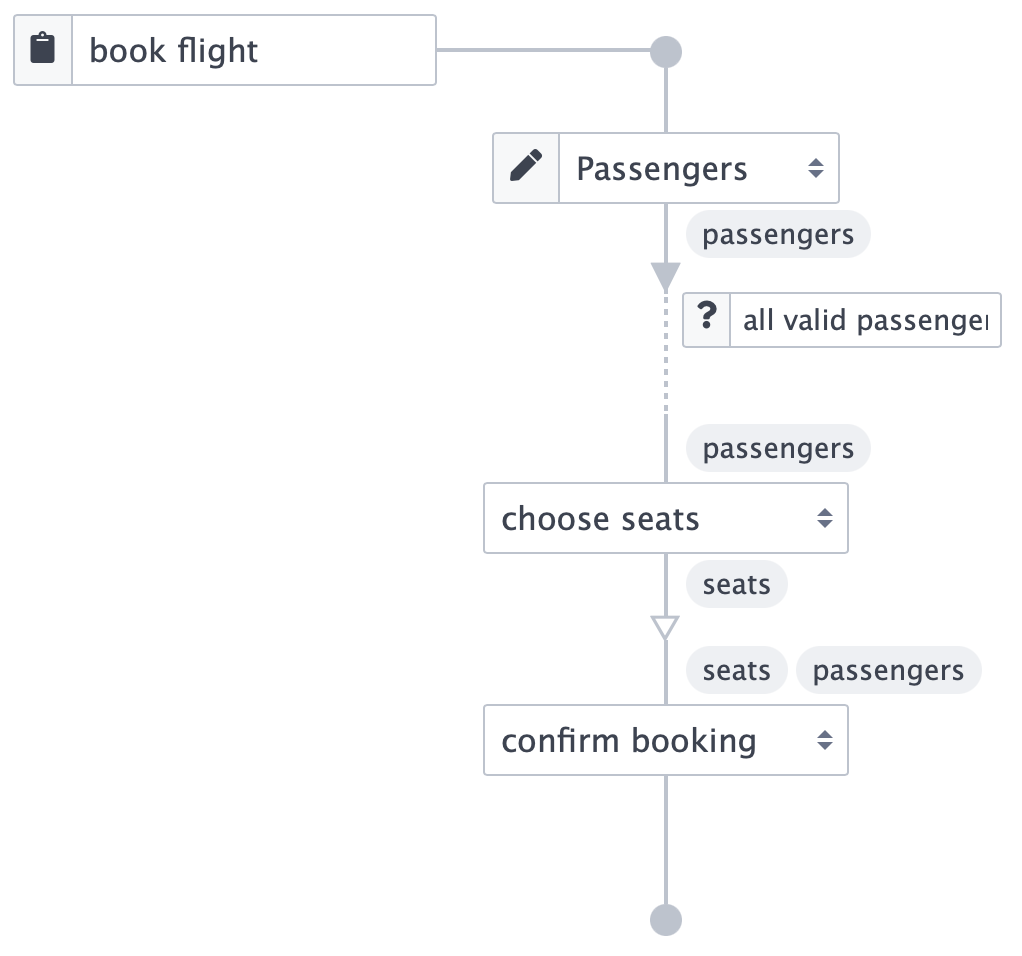
\includegraphics[width=\columnwidth]{figures/flight-booking.png}
    \caption{Running web application of the flight booking example using an elaboration into \ITASKS.}
    %  It shows three users booking a flight simultaneously.
    %  The first user entered name and age and continued picking seats.
    %  The second is entering details of two passengers.
    %  The ages are not filled in, therefore the \var{Continue} button is disabled.
    %  The message bubble shows that the \var{age} field only accepts integer values.
    %  The third user finished a booking,
    %  therefore, the first user can not pick seats \smallcaps{1b} and \smallcaps{1c} any more.}
  \end{figure}

  We can run this program by translating above \TOPHAT\ code to \ITASKS.
  % \cref{app:itasks} gives an overview of equivalent constructs in both systems.
  A screenshot of the resulting web application is shown in \cref{fig:flight-booking}.

  All instances of the \var{bookFlight} task have access to the shared list of free seats.
  Rewriting the example in a language without references would not only be cumbersome,
  % obfuscating the code with explicit threading of state,
  but it would be impossible to model the parallel execution of three \var{bookFlight} tasks.
  It is not known upfront which task will finish first,
  and thus it is not possible to thread the free seat list itself between the parallel tasks.
\end{example}

% \begin{TASK}[emph={passengers,chosen,free}]
%   let main =
%     share [(1, 'A'), (1, 'B'), (2, 'A'), (2, 'B'), ...] >>= do free.
%     watch free <&> >&<$_\text{\var{book \emph{free}}}$ []

%   let book = do free.
%     enter List Passenger >>= do passengers.
%       all valid passengers |->
%         choose_seats passengers free >>= do chosen.
%         confirm_booking passengers chosen >>= do _.
%         assert length passengers == length chosen
%         assert unique chosen
%         assert chosen /< free

%   let choose_seats = do passengers. do free.
%     (watch free <&> enter Seats) >>= do (free, chosen).
%     intersect chosen free /\ length passengers == length chosen
%       |-> confirm_booking passengers chosen free

%   let confirm_booking = do passengers. do chosen. do free.
%     free ::= difference chosen
%     view (passengers, chosen)
% \end{TASK}

%   % allValid :: Passengers -> Bool
%   % allValid ps = all isValid ps && any isAdult ps

%   % isValid :: Passenger -> Bool
%   % isValid (n, a) = n /= "" && a >= 0

%   % isAdult :: Passenger -> Bool
%   % isAdult (_, a) = a >= 18

%   % isCorrect :: Seats -> Seats -> Bool
%   % isCorrect ss fs = do
%   %   List.intersect ss fs == ss

% \begin{TASK}[emph={passengers,seats,free}]
%   let book_flight = do free.
%     enter List Passenger >>= do passengers.
%       all valid passengers |->
%         choose_seats passengers >>= do seats.
%         confirm_booking passengers seats
%         assert length passengers == length seats
%         assert unique seats
%         assert seats /< free
% \end{TASK}

% \begin{TASK}[emph={passengers,seats,free}]
%   book_flight free <&> book_flight free
% \end{TASK}

% \begin{TASK}[emph={passengers,seats,free}]
%   let main =
%     book_flight free
%           <&>
%     book_flight free
%           <&>
%     book_flight free
%           <&>
%            $\vdots$
% \end{TASK}

% \begin{TASK}[emph={passengers,seats,free}]
%   let main =
%     >&<$_\text{\var{book\_flight \emph{free}}}$ []
% \end{TASK}
% \begin{TASK}[emph={passengers,seats,free}]
%   let main =
%     >&<$_\text{\var{book\_flight \emph{free}}}$ [book_flight free]
% \end{TASK}
% \begin{TASK}[emph={passengers,seats,free}]
%   let main =
%     >&<$_\text{\var{book\_flight \emph{free}}}$ [choose_seats ..., book_flight free]
% \end{TASK}
% \begin{TASK}[emph={passengers,seats,free}]
%   let main =
%     >&<$_\text{\var{book\_flight \emph{free}}}$ [choose_seats ...]
% \end{TASK}
\section{Properties}
\label{sec:properties}

% !TEX root=../main.tex

\subsection{Symbolic execution}

Previous work introduces a symbolic execution semantics for \TOPHAT\ programs~\cite{conf/ifl/NausSK19}. \todo{moeten we hier jou en/of mijn proefschrift ook nog citen? Zie ook beneden}
By defining semantic rules that introduce symbols where user input is expected, the behavior of a TOP program can be fully described.
This symbolic behavior description can then be used to reason over the properties of the program. 
Figure~\ref{fig:symbolic-semantics} lists a selected number of symbolic execution rules.
\todo{insert rules and describe them in some level of detail.}

\begin{figure}
    TODO TODO TODO
    \caption{Examples of symbolic execution rules for \TOPHAT}
    \label{fig:symbolic-semantics}
\end{figure}

Ultimately, the symbolic execution of a \TOPHAT\ program is then powered by a top-level simulation function, that leverages the symbolic rules to perform symbolic execution.
Since a user can update an editor as often as they want, special care is taken to ensure that only \textit{productive} updates are generated by the symbolic execution function.
An editor can only be updated twice, if the task, modulo the updated value, has changed.
This allows exactly enough repetition to capture the full program behavior.
For example, the second task in a parallel composition might rely on a value being updated in the first task, to make progress. \todo{wil je hier ook de simulate functie laten zien?}

When it comes to \DYNTOPHAT, there is an additional opportunity for infinite interaction, namely to spool up a new task.
Unfortunately, in this case, there is no way to set an upper bound on this interaction without changing the program's behavior.
Imagine we have a task pool combinator, followed by a step.
We restrict the number of new task initializations to be no larger than some $n$.
The step could very well require $n+1$ values before it will allow a step.
It is clear from this example that limiting task initialization is not a suitable way to deal with the infinite interaction coming from the pool combinator.

The pool combinator breaks traditional symbolic execution as introduced in previous work~\cite{conf/ifl/NausSK19}.
That does not mean that the symbolic execution of \DYNTOPHAT\ programs is now completely useless.
Built on top of the symbolic execution engine, \citet{conf/sfp/NausS20} presents a system that assists users of \TOPHAT\ programs in finding the next input action to perform.
The basic idea is that symbolic execution can be leveraged to reach some goal $g$.
Figure~\ref{fig:next-step-hint} defines a function that calculates these so-called next-step-hints.

\begin{figure}
    TODO TODO TODO
    \caption{Next-step hint generation function}
    \label{fig:next-step-hint}
\end{figure}

\todo{explain the function in this figure, and how it uses symbolic execution.}

The addition of a symbolic execution rule for the task pool combinator breaks the definition from Figure~\ref{fig:next-step-hint}, since the symbolic interaction \textit{traces} are now potentially infinite. \todo{add a symbolic rule for task pool combinator}
Instead of calculating all possible hints, one could alter the hints function to perform a breadth-first search through the now infinite trace space.
This allows us to return a hint that guides the user to the shortest path to their goal.
Figure~\ref{fig:next-step-hint-pool} lists an updated definition of the next-step hint function.

\begin{figure}
    TODO TODO TODO
    \caption{Next-step hint generation function}
    \label{fig:next-step-hint-pool}
\end{figure}

Coming back to reasoning about task properties, the breadth-first search strategy can also be applied to finding assertion violations.
\citet{DBLP:conf/tap/NausVSR23} demonstrate a breadth-first search approach to finding assertion violations in low-level programs with potential infinite search spaces.
This approach can also be applied to \DYNTOPHAT\ programs, using the insights described above.

To conclude, adding task pools to \TOPHAT\ does restrict the use of symbolic execution, but it still has several viable applications.
These restrictions are similar to those found with any real-world application of symbolic execution.
A more extensive discussion on this point can be found elsewhere~\cite{conf/ifl/NausSK19}.
\newmacro{citeprop}[1]{[Prop.~#1]} % {\cite[Prop.~#1]{conf/sfp/KlijnsmaS22}}

\subsection{Task equivalence}
\label{sec:equivalence}

We do this by categorizing tasks based on the observations we can make on them.
The observations we use, are if the task is failing ($\Failing$), if the task can receive any inputs ($\Inputs$), and if the task has a value ($\Value$).
Based on these three observations, a (fully fixated) task can be in one of five \emph{conditions} which we will summarise below.
The mentioned properties are proved in \citet{conf/sfp/KlijnsmaS22}.
We refer to the propositions \todo{}.

\begin{description}

  \item[Failing]
    A failing task $t$ is a task for which the failing function $\Failing(t)$ yields true.
    If a task is failing, we can prove that it accepts no more use input and has no value \citeprop{12}.
    That is, $\Inputs(t) = \empty$ and $\Value(t,\sigma) = \bot$.
    We also know that, if $\Failing(t) = \True$, it stays failing \citeprop{1},
    simply because there is no input which can rewrite $t$ to another $t'$.
    % We have proven this property in \todo{} in the appendix.

  \item[Stuck]
    A stuck task $t$ is a task which does not fail, does not accept user input, and does not have a value.
    That is, $\Failing(t) = \False$, $\Inputs(t) = \empty$, and $\Value(t,\sigma) = \bot$.
    Similar to failing tasks, stuck tasks will always remain stuck because no more user interaction is possible and, by assumption, it is already fully fixated \citeprop{3}.

  \item[Steady]
    If a task $t$ has a value but it cannot handle any input, we call it \emph{steady}.
    An example of a steady task is $\View^k 42$.
    Because this task accepts no more user input, its value will always remain equal to $42$.

  \item[Unsteady]
    If a task $t$ has a value and it can handle input, we call it \emph{unsteady}.
    An example of an unsteady task is $\Update^k 42$.
    This task still accepts user input, and thus its value can keep on changing.
    Even though this example and $\View^k 42$ yield the same value,
    they should not be equivalent, since one's value can be changed and the other one's value cannot.
    If a task $t$ is unsteady, it will never terminate: an unsteady task will always remain unsteady with the same input space, only its value may change \citeprop{2}.

  \item[Running]
    The last condition is when a task $t$ does not fail, does not have a value, but still accepts user input.
    Because there is still user interaction possible, it may be the case that with the right input, it transitions to one of the previously described task conditions.
    The simplest example of a running task is the empty editor $\Enter^k \beta$, which becomes an unsteady task once it receives a valid input event.
    Although running tasks can keep running forever,
    we at least can prove that they will not fail \citeprop{4}.

\end{description}

These conditions are mutually exclusive \citeprop{5}.

\begin{table}
  \begin{tabular}{CCClL}
  \toprule
  \Failing   & \Inputs    & \Value     & \alert{Condition} & \alert{Examples}                                                                                                             \\
  \midrule
  \checkmark & -          & -          & Failing           & \Fail, \,\, \Fail \Pair \Fail, \,\, (\lambda x.x) \Trans \Fail, \,\, \Fail \Step \lambda x.\View x \\
  -          & -          & -          & Stuck             & \View 2 \Step \lambda x.\Fail, \,\, \View 2 \Pair \Fail, \,\, \Fail \Pair \View 2                                            \\
  -          & -          & \checkmark & Steady            & \View 2, \,\, \View 2 \Pair \View 3, \,\, \View \tuple{2, 3}                          \\
  -          & \checkmark & \checkmark & Unsteady          & \Update 2, \,\, \Update 2 \Pair \Update 3, \,\, \Update \tuple{2, 3}                                                         \\
  -          & \checkmark & -          & Running           & \Enter \Int \Pair \Fail, \,\, \Update 2 \Step \lambda x.\Fail                                                                \\
  \bottomrule
\end{tabular}
\\
{\small
  Checkmarks for $\Failing$, $\Value$ and $\Inputs$ for a task $t$ and a state $\sigma$ indicate that\\
  $\Failing(t) = \True$,
  $\Value(t, \sigma) = v$ for $v \neq \bot$, and
  $\Inputs(t) \neq \nothing$ respectively.
}

  \caption{Conditions for tasks}
  \label{tab:task-conditions}
\end{table}

\begin{figure}
  \begin{tikzpicture}[x=1pc,y=1pc,shorten >=1pt,minimum size=3.5pc,node distance={0.33pc and 3pc},>={Triangle},draw=black,thick]
  \node[circle,draw,very thick] (running)                            {\emph{Running}};
  \node[circle,draw,very thick] (failing)   [above left=of running]  {\emph{Failing}};
  \node[circle,draw,very thick] (stuck)     [above right=of running] {\emph{Stuck}};
  \node[circle,draw,very thick] (finished)  [below left=of running]  {\emph{Steady}};
  \node[circle,draw,very thick] (recurring) [below right=of running] {\emph{Unsteady}};
  %
  % \draw[thick,->] (running) -- (failing);
  \draw[->] (running) -- (finished);
  \draw[->] (running) -- (recurring);
  \draw[->] (running) -- (stuck);
  \draw[->] (recurring) edge [out=423,in=387,looseness=6]  (recurring);
  \draw[->] (running) edge [out=108,in=72,looseness=6]  (running);
\end{tikzpicture}

  \caption{Possible task conditions and their transitions, where a transition is caused by user interaction ($\interact{\iota}$) for some input $\iota$.}
  \label{fig:task-conditions}
\end{figure}


---------






Propositions from \cite{Steenvoorden22} and \cite{Klijnsma2020} that still hold are the following:

\begin{itemize}
  \item Valued tasks are static
  \item Steady tasks stay steady
\end{itemize}

However, because of the dynamic nature of task pools, the following propositions need alteration:

\begin{itemize}
  \item Static tasks stay static
  \item Finished tasks stay finished
\end{itemize}

This is because task pools can always receive the initialise input ($\Init$),
so tasks containing a task pool will never get to a steady state!

We will discuss the impact on equational reasoning on tasks more thoroughly...
\subsection{Task visualisation}

\todo{write section}

% !TEX root=../main.tex

\section{Related Work}

TOP has been studied for a long time:

executable specifications of interactive work flow systems for the web~\cite{conf/icfp/PlasmeijerAK07}
TOP in a pure functional language~\cite{conf/ppdp/PlasmeijerLMAK12}
distributed top~\cite{conf/ifl/OortgieseGAP17}

These implementations lack a formal foundation, making it harder to reason about stuff like correctness, equivalence, valuation, etc.

tophat~\cite{conf/ppdp/SteenvoordenNK19}

This formal foundation has lead to development of formal methods in TOP:

symbolic tophat~\cite{conf/ifl/NausSK19}
top with feedback~\cite{conf/sfp/NausS20}
Equivalence of programs~\cite{DBLP:conf/sfp/KlijnsmaS22}




% !TEX root=../main.tex

\section{Conclusion}
\label{sec:conclusion}

We presented the problem that programmers need to specify the number of parallel tasks in \TOPHAT\ during development time
and introduced \emph{task pools} as a solution.
In the resulting language \DYNTOPHAT\ is a moderate extension to \TOPHAT\ with more dynamic properties.
At runtime, end-users can initialise and kill tasks in a pool at will.
We presented the static and dynamic semantics of task pools extending \TOPHAT\ multiple semantic layers.
We were able to do this in such a way that the impact on formal reasoning of \TOPHAT\ programs is minimal.
Although symbolic execution could end in an infinite loop,
we altered our next-step hint generation system so that it can still support end-users during workflow execution.
Also, our semantic extensions were defined in such a way, that equational reasoning on tasks is still possible
and transformation laws proved in earlier work still hold.

This reinforces our belief that the given definitions and semantics for task pools are the right choice.

% !TEX root=../main.tex

\section{Discussion}

\paragraph{Future work}
\label{sec:future-work}

In the future, we would like to investigate the amount of real-world tasks written in \ITASKS\ that could be rewritten by using task pools.
This way, such tasks could benefit from validation by symbolic execution without compromising expressivity.
Also, developers could use the transformation rules from \citet{conf/sfp/KlijnsmaS22} to refactor their programs.

It would be even more interesting, however, when task pools will fall short in these real-world examples.
In that case, we would like to investigate which additional power is needed in \TOPHAT\ to write these programs and reason about them.


\begin{acks}
  % !TEX root=../main.tex

\end{acks}

%% The next two lines define the bibliography style to be used, and
%% the bibliography file.
\bibliographystyle{ACM-Reference-Format}
\bibliography{dblp,other}


\end{document}
\endinput
%%
%% End of file `sample-authordraft.tex'.
